% ======================================================================
% PREÁMBULO
% ======================================================================
\documentclass[12pt,a4paper]{article}
\usepackage[utf8]{inputenc}
\usepackage[spanish]{babel}
\usepackage{graphicx}
\usepackage{geometry}
\geometry{a4paper, margin=2cm}
\usepackage{hyperref}
\usepackage{float}
\usepackage{longtable}
\usepackage{array}

% Configuración de hyperref
\hypersetup{
    colorlinks=true,
    linkcolor=black,
    urlcolor=blue,
    citecolor=black
}

% ======================================================================
% PORTADA
% ======================================================================
\title{\textbf{Proyecto Final: Bases de Datos Avanzadas}\\Sistema de Gesti\'on para Centro de Salud}
\author{
    Diego David Chinchilla Leal \\ C\'odigo: 20221578047 \\[0.3cm]
    Miguel Angel Cardenas Monta\~nez \\ C\'odigo: 20202578003 \\[0.3cm]
    Michael David Garz\'on Rodr\'iguez \\ C\'odigo: 20261678063
}
\date{}

\begin{document}

\maketitle

\begin{center}
    \textbf{Universidad:} Universidad Distrital Francisco Jos\'e de Caldas \\
    \textbf{Materia:} Bases de Datos Avanzadas \\
    \textbf{Docente:} Claudia Liliana Hern\'andez Garc\'ia \\
    \textbf{Grupo:} 303 \\
    \textbf{Fecha:} \today
\end{center}

% ======================================================================
% TABLA DE CONTENIDOS
% ======================================================================
\newpage
\tableofcontents
\newpage

% ======================================================================
% SECCIÓN 1: DEFINICIÓN DEL PROBLEMA
% ======================================================================
\section{Definici\'on del Problema}

\subsection{a) Descripci\'on de funcionalidades (aplicaci\'on)}

El centro de salud necesita un sistema para gestionar toda su informaci\'on: m\'edicos, empleados, pacientes, horarios, vacaciones, sustituciones y diagn\'osticos. Actualmente todo se maneja en papel o en hojas de Excel, lo que genera p\'erdida de informaci\'on, registros duplicados y dificultad para consultar datos hist\'oricos. La soluci\'on propuesta permite que cada persona pueda consultar y registrar lo que le corresponde, evitando duplicidad, p\'erdida de datos e inconsistencias.

En la siguiente tabla se resumen las funcionalidades principales que va a tener el sistema:

{\footnotesize
\setlength{\tabcolsep}{4pt}
\begin{longtable}{|p{2.3cm}|p{3.5cm}|p{2.2cm}|p{2cm}|p{1.2cm}|p{2.8cm}|}
\hline
\textbf{Funcionalidad} & \textbf{Descripci\'on} & \textbf{Datos Requeridos} & \textbf{Datos Mostrados} & \textbf{Usuario} & \textbf{Reglas Asociadas} \\ \hline
\endfirsthead
\hline
\textbf{Funcionalidad} & \textbf{Descripci\'on} & \textbf{Datos Requeridos} & \textbf{Datos Mostrados} & \textbf{Usuario} & \textbf{Reglas Asociadas} \\ \hline
\endhead

Gesti\'on de M\'edicos &
Permite registrar nuevos m\'edicos, consultar su informaci\'on, modificar datos cuando sea necesario y desactivarlos si ya no trabajan en el centro &
Datos personales, n\'umero de licencia, especialidad, tipo de vinculaci\'on &
Ficha completa del m\'edico con toda su informaci\'on &
Admin / RRHH &
Cada m\'edico debe tener un solo tipo (titular, interino o sustituto). La licencia m\'edica debe ser \'unica en el sistema. \\ \hline

Gesti\'on de Horarios &
Permite asignar los turnos de consulta de cada m\'edico, estableciendo en qu\'e d\'ias y a qu\'e horas atiende pacientes &
D\'ia de la semana, hora de inicio, hora de fin, m\'edico asociado &
Horario semanal del m\'edico con los turnos asignados &
Admin &
Un m\'edico puede tener horarios diferentes cada d\'ia de la semana. No pueden existir horarios que se traslapen para el mismo m\'edico. \\ \hline

Control de Sustitutos &
Administra el historial completo de los periodos en los que un m\'edico sustituto ha trabajado en el centro, registrando sus fechas de ingreso y retiro &
M\'edico sustituto, fecha de ingreso, fecha de retiro &
Historial de sustituciones con fechas y estado actual &
RRHH &
Cuando un sustituto termina no se borra su informaci\'on, solo se registra la fecha de retiro. El estado de \"activo\" se determina comparando las fechas. \\ \hline

Gesti\'on de Empleados &
Permite administrar la informaci\'on del personal que no es m\'edico, como auxiliares, vigilantes y personal administrativo &
Datos personales, profesi\'on, municipio &
Ficha completa del empleado &
RRHH &
Cada empleado debe pertenecer a una de las profesiones definidas en el sistema. \\ \hline

Gesti\'on de Vacaciones &
Controla los periodos vacacionales de todo el personal, tanto m\'edicos como empleados, registrando las fechas de inicio y fin &
Empleado, fecha de inicio, fecha de fin &
Periodos vacacionales registrados y su estado actual &
RRHH &
El estado de las vacaciones (planificadas o disfrutadas) se calcula autom\'aticamente comparando las fechas con la fecha actual del sistema. \\ \hline

Gesti\'on de Pacientes &
Mantiene el registro de todos los pacientes del centro, sus datos personales y la asignaci\'on del m\'edico responsable de cada caso &
Datos personales, municipio, m\'edico asignado &
Ficha del paciente con su m\'edico a cargo &
M\'edico / Admin &
Cada paciente debe tener un \'unico m\'edico responsable. Un m\'edico puede tener varios pacientes a su cargo. \\ \hline

Gesti\'on de Diagn\'osticos &
Permite registrar los diagn\'osticos m\'edicos de cada paciente a lo largo del tiempo, llevando un historial cronol\'ogico &
Paciente, fecha del diagn\'ostico, descripci\'on &
Lista de diagn\'osticos del paciente ordenados por fecha &
M\'edico &
Un paciente puede tener varios diagn\'osticos en distintas fechas. Cada diagn\'istico debe tener una descripci\'on detallada. \\ \hline

Gesti\'on de Reportes &
Genera los listados solicitados en el enunciado del proyecto: pacientes por m\'edico, m\'edicos por especialidad, diagn\'osticos por enfermedad y vacaciones del personal &
Criterios de b\'usqueda (especialidad, enfermedad, rango de fechas) &
Resultados en formato tabular &
Gerencia &
Debe cumplir con los cuatro reportes exigidos en el enunciado del proyecto. \\ \hline

Acceso al Sistema &
Controla el inicio de sesi\'on mediante usuario y contrase\~na, y redirige a cada persona seg\'un su rol (admin, m\'edico, enfermero o recepcionista) &
Nombre de usuario, contrase\~na &
Pantalla principal del rol correspondiente &
Todos &
Cada usuario debe tener un rol asignado. Las contrase\~nas se almacenan de forma segura usando hash SHA-256. \\ \hline

Gesti\'on de Usuarios &
Permite crear, editar y desactivar cuentas de usuario del sistema, as\'ignando nombre de usuario, contrase\~na, rol y estado activo/inactivo &
Nombre de usuario, contrase\~na, rol, nombre completo &
Lista de usuarios con su rol y estado &
Admin &
Solo el administrador puede gestionar usuarios. No se puede eliminar un usuario, solo desactivarlo. \\ \hline

Historial del Paciente &
Muestra el historial cl\'inico completo de un paciente, con todos sus diagn\'osticos ordenados cronol\'ogicamente y qui\'en los registr\'o &
Paciente seleccionado &
Lista de diagn\'osticos con fecha, descripci\'on y usuario que lo registr\'o &
M\'edico / Admin &
\caption{Funcionalidades del sistema de gesti\'on para centro de salud}
\end{longtable}
}

\newpage

\subsection{b) Descripci\'on del entorno de ejecuci\'on (S.O., Motor de BD)}

Para este proyecto seleccionamos cada herramienta con base en los requisitos t\'ecnicos y el contexto del centro de salud:

\begin{itemize}
    \item \textbf{Sistema Operativo -- Windows 10/11:} Se eligi\'o Windows por ser el sistema operativo m\'as extendido en centros de salud y consultorios m\'edicos en Colombia, lo que facilita el soporte t\'ecnico y la capacitaci\'on del personal. Adem\'as, Windows ofrece compatibilidad completa con MySQL Server 8.0 y las herramientas de desarrollo utilizadas, sin necesidad de configuraciones adicionales de compatibilidad.

    \item \textbf{Motor de Base de Datos -- MySQL 8.0:} MySQL se seleccion\'o por las siguientes razones t\'ecnicas: (1) es un motor relacional maduro que soporta completamente disparadores (triggers), procedimientos almacenados, vistas y restricciones CHECK, caracter\'isticas exigidas en el enunciado del proyecto; (2) cuenta con licencia gratuita (Community Edition) que no genera costos de implementaci\'on; (3) ofrece conectividad nativa con Python a trav\'es del conector oficial mysql-connector-python, y (4) su amplia adopci\'on en el \'mbito acad\'emico garantiza disponibilidad de documentaci\'on y soporte.

    \item \textbf{Herramientas de Desarrollo:}
    \begin{itemize}
        \item \textit{MySQL Workbench 8.0:} Se emple\'o para el modelado conceptual y relacional de la base de datos, la generaci\'on de los diagramas ER y relacional, y la administraci\'on visual del esquema. Su motor de reverse engineering permite exportar el diagrama directamente desde la base de datos implementada, garantizando que el modelo gr\'afico refleje fielmente la estructura f\'isica.

        \item \textit{Visual Studio Code:} Se utiliz\'o como entorno de desarrollo integrado por su ligereza, soporte nativo para Python y Git, y su ecosistema de extensiones que facilitan la edici\'on de c\'odigo, la depuraci\'on y el control de versiones.

        \item \textit{Python 3.x con Streamlit:} Python se seleccion\'o como lenguaje de programaci\'on por su sintaxis clara y su amplio soporte para conectividad con bases de datos. Streamlit, espec\'ificamente, permite construir interfaces web interactivas (formularios, tablas, gr\'aficos) escribiendo \'unicamente c\'odigo Python, sin necesidad de HTML, CSS o JavaScript. Esto aceler\'o el desarrollo de la aplicaci\'on de escritorio-web del centro de salud.
    \end{itemize}
\end{itemize}

\subsection{c) Definici\'on de las reglas de negocio (delimitar problema)}

A continuaci\'on se presentan las reglas que rigen el funcionamiento del centro de salud. Estas reglas fueron definidas pensando en c\'omo se maneja la informaci\'on d\'ia a d\'ia en el centro, usando un lenguaje natural y evitando los t\'erminos t\'ecnicos de bases de datos.

\begin{itemize}

    \item \textbf{Tipos de m\'edicos.} En el centro de salud hay m\'edicos de tres tipos: los que tienen un contrato fijo (titulares), los que est\'an reemplazando temporalmente a un compa\~nero que est\'a ausente (interinos) y los que cubren ausencias cuando se necesita (sustitutos).

    \item \textbf{Historial de sustitutos.} Cuando un m\'edico sustituto termina su labor no se borra su informaci\'on del sistema, sino que se le registra una fecha de retiro. De esta manera se puede consultar el historial completo de todas las veces que ha trabajado en el centro. Si la \'ultima fecha de ingreso es posterior a la \'ultima fecha de retiro (o no hay fecha de retiro registrada), quiere decir que el m\'edico est\'a trabajando actualmente en el centro.

    \item \textbf{M\'edicos como empleados.} Todos los m\'edicos tambi\'en son empleados del centro, as\'i que comparten datos b\'asicos como el nombre, la direcci\'on y el municipio donde viven. Adem\'as de estos datos, los m\'edicos tienen informaci\'on adicional como su n\'umero de licencia, la especialidad en la que trabajan y el tipo de vinculaci\'on que tienen con el centro.

    \item \textbf{Personal no m\'edico.} Los dem\'as empleados del centro que no son m\'edicos pueden ser auxiliares de enfermer\'ia, vigilantes o personal administrativo. Cada uno de ellos tiene una profesi\'on espec\'ifica que los identifica dentro del centro.

    \item \textbf{Asignaci\'on de pacientes.} Cada paciente tiene un \'unico m\'edico que se encarga de su caso. Sin embargo, un mismo m\'edico puede atender a varios pacientes al mismo tiempo, sin l\'imite definido.

    \item \textbf{Vacaciones del personal.} Cualquier trabajador del centro, ya sea m\'edico o de otro tipo, puede solicitar vacaciones. El sistema guarda la fecha de inicio y la fecha de fin de cada periodo vacacional. Seg\'un la fecha actual, el sistema puede determinar si las vacaciones ya se disfrutaron (si la fecha de fin ya pas\'o) o si todav\'ia est\'an planeadas (si la fecha de inicio es futura).

    \item \textbf{Tel\'efonos de contacto.} Tanto los pacientes como los empleados pueden tener m\'as de un n\'umero de tel\'efono registrado para que los contacten. Esto es \'util cuando una persona tiene un tel\'efono fijo y un celular, por ejemplo.

    \item \textbf{Diagn\'osticos a trav\'es del tiempo.} Un paciente puede tener varios diagn\'osticos a lo largo del tiempo porque asiste al m\'edico en distintas ocasiones. Cada diagn\'istico queda registrado con su fecha y una descripci\'on detallada, formando as\'i el historial cl\'inico del paciente.

\item \textbf{Validaciones para evitar errores en los registros.} No se debe permitir que un m\'edico tenga dos turnos que se empalmen en el mismo d\'ia, porque no puede atender dos consultas al mismo tiempo. Un empleado no puede tener dos periodos de vacaciones que se crucen entre s\'i. \'Unicamente los m\'edicos que trabajan como sustitutos pueden tener periodos de sustituci\'on registrados. Tampoco se puede registrar un diagn\'ostico con una fecha futura, porque corresponder\'ia a una atenci\'on que a\'un no ha ocurrido.

\item \textbf{Disponibilidad m\'edica.} Un m\'edico se considera disponible para atender pacientes cuando pertenece a la especialidad solicitada, no se encuentra actualmente de vacaciones y, en caso de ser sustituto, tiene un periodo de sustituci\'on activo. Para los sustitutos, se toma como referencia el \'ultimo periodo registrado: si la fecha de ingreso ya ocurri\'o y la fecha de retiro es nula o a\'un no ha llegado, el sustituto se considera activo.

\item \textbf{Asignaci\'on segura de pacientes.} No se deben asignar pacientes nuevos a m\'edicos que en ese momento no est\'en disponibles para atender, como los que est\'an de vacaciones o los m\'edicos sustitutos que no tienen un periodo activo en el centro.

\item \textbf{Auditor\'ia de operaciones.} Para mejorar la trazabilidad del sistema, se registra una bit\'acora cuando se crean datos cl\'inicos o administrativos relevantes, como pacientes, diagn\'osticos y vacaciones. Esto permite conocer qu\'e tabla fue afectada, qu\'e operaci\'on se realiz\'o y en qu\'e momento ocurri\'o.

\end{itemize}

\vspace{0.5cm}

\subsection{Matriz de cumplimiento de solicitudes del enunciado}

La siguiente tabla relaciona cada solicitud del enunciado con el objeto de base de datos y el módulo de la aplicación que permite resolverla. Esto permite verificar que la solución cubre los requerimientos funcionales del centro de salud.

{\small
\begin{longtable}{|p{5cm}|p{4cm}|p{5cm}|}
\hline
\textbf{Solicitud del enunciado} & \textbf{Objeto SQL} & \textbf{Módulo de la aplicación} \\ \hline
\endfirsthead
\hline
\textbf{Solicitud del enunciado} & \textbf{Objeto SQL} & \textbf{Módulo de la aplicación} \\ \hline
\endhead

Listado de pacientes a cargo de un médico según su especialidad & vw\_pacientes\_medicos y sp\_pacientes\_por\_especialidad & Reportes del Centro: Pacientes por especialidad \\ \hline

Listado de médicos disponibles para una especialidad particular & vw\_medicos\_info y sp\_medicos\_disponibles\_por\_especialidad & Reportes del Centro: Médicos disponibles \\ \hline

Datos de pacientes diagnosticados con una enfermedad específica & vw\_diagnosticos\_pacientes y sp\_pacientes\_por\_diagnostico & Reportes del Centro: Pacientes por diagnóstico \\ \hline

Médicos que han disfrutado o planean vacaciones en un intervalo & vw\_vacaciones\_medicos y sp\_vacaciones\_medicos\_intervalo & Reportes del Centro: Vacaciones por intervalo \\ \hline

\caption{Matriz de cumplimiento del enunciado}
\end{longtable}}

% ======================================================================
% SECCIÓN 2: DIAGRAMA DEL MODELO ENTIDAD RELACIÓN
% ======================================================================
\newpage
\section{Diagrama del Modelo Entidad Relaci\'on}

El diagrama que se muestra a continuaci\'on es el modelo conceptual que hicimos para representar c\'omo se relacionan las cosas del centro de salud. De ah\'i sali\'o toda la base de datos, ah\'i se ven las entidades y c\'omo se conectan entre s\'i.

\begin{figure}[H]
    \centering
    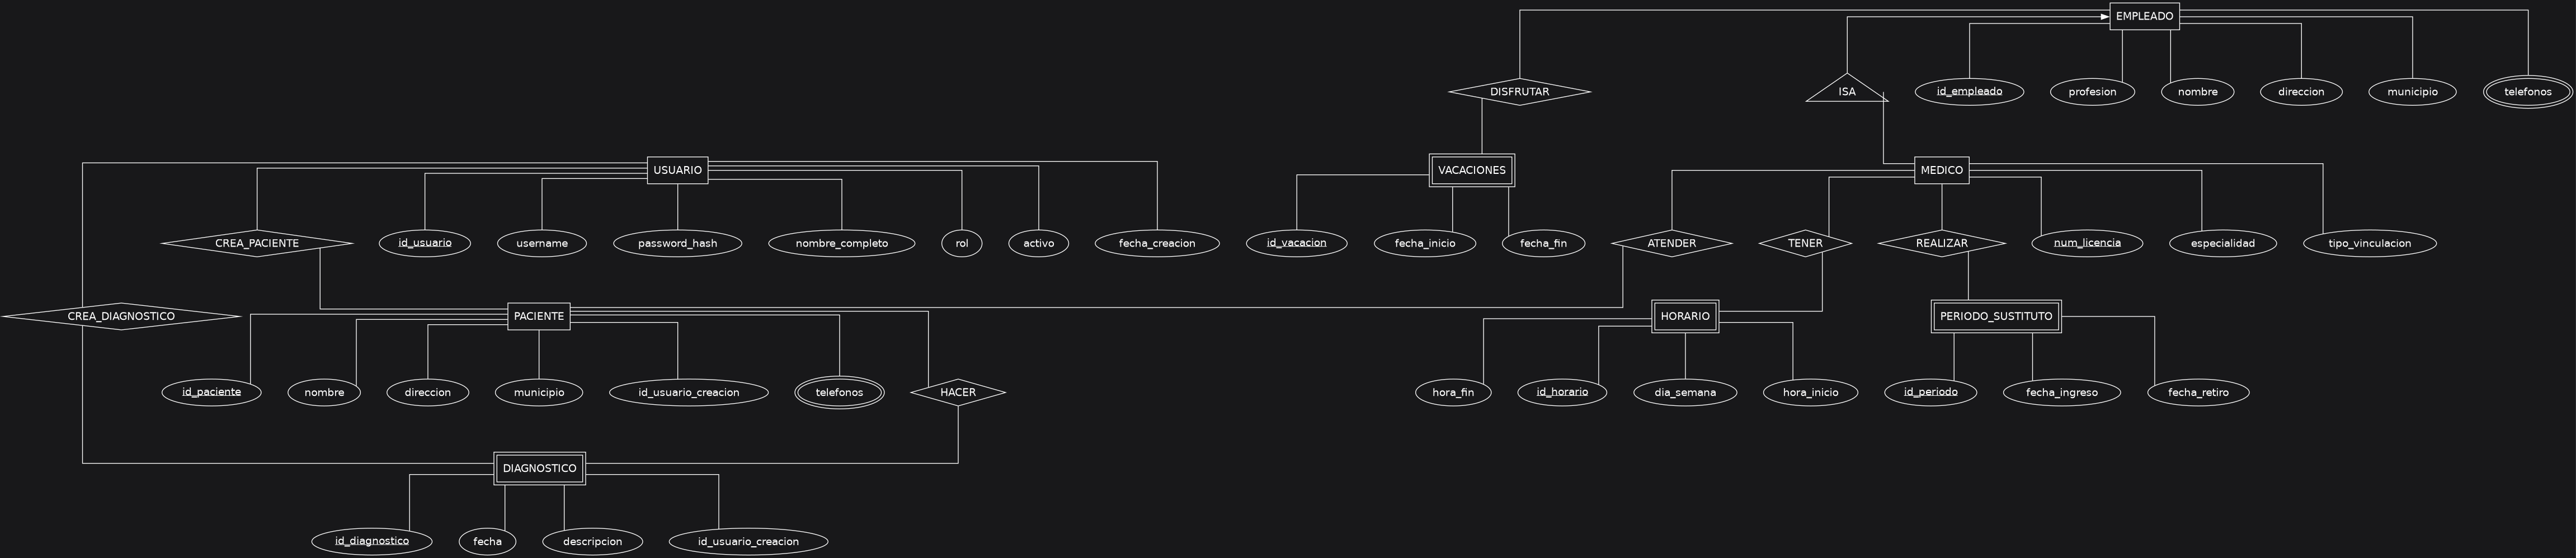
\includegraphics[width=1.0\textwidth]{Diagrama_ER_Oscuro_Normalizado.png}
    \caption{Diagrama del Modelo Entidad-Relaci\'on Conceptual}
    \label{fig:er_conceptual}
\end{figure}

A continuaci\'on se describen los elementos principales del diagrama:

\begin{itemize}
    \item \textbf{L\'ineas ortogonales:} Las conexiones entre entidades se hicieron con l\'ineas rectas (horizontales y verticales) para que el diagrama se vea m\'as limpio y no tan desordenado.

    \item \textbf{Generalizaci\'on entre EMPLEADO y MEDICO:} En el diagrama se ve un tri\'angulo ISA que conecta EMPLEADO con MEDICO. B\'asicamente significa que los m\'edicos son empleados pero con datos extra como la licencia y la especialidad.

    \item \textbf{Entidades d\'ebiles:} Las entidades HORARIO, PERIODO\_SUSTITUTO, VACACIONES y DIAGN\'OSTICO aparecen con doble recuadro (periferias=2) porque su existencia depende completamente de otra entidad. Un horario no tiene sentido si no est\'a asociado a un m\'edico concreto; un periodo de sustituci\'on solo existe si hay un m\'edico sustituto que lo ejecuta; las vacaciones siempre pertenecen a un empleado espec\'ifico, y un diagn\'ostico siempre est\'a vinculado a un paciente. En todos estos casos, la entidad fuerte correspondiente (EMPLEADO, MEDICO o PACIENTE) define el contexto de existencia de la entidad d\'ebil, y sin ella el registro carecer\'ia de significado.

    \item \textbf{Sin atributo ``estado'' en VACACIONES:} La profe nos pidió quitar el campo ``estado'' de las vacaciones. Ahora el estado se calcula autom\'aticamente comparando las fechas con la fecha de hoy.
\end{itemize}

% ======================================================================
% SECCIÓN 3: DIAGRAMA DEL MODELO RELACIONAL
% ======================================================================
\newpage
\section{Diagrama del Modelo Relacional}

El diagrama relacional representa la estructura f\'isica de las tablas, sus columnas, tipos de dato y relaciones en MySQL. Aqu\'i se puede ver c\'omo quedaron las tablas del modelo relacional implementadas en el motor de base de datos.

\begin{figure}[H]
    \centering
    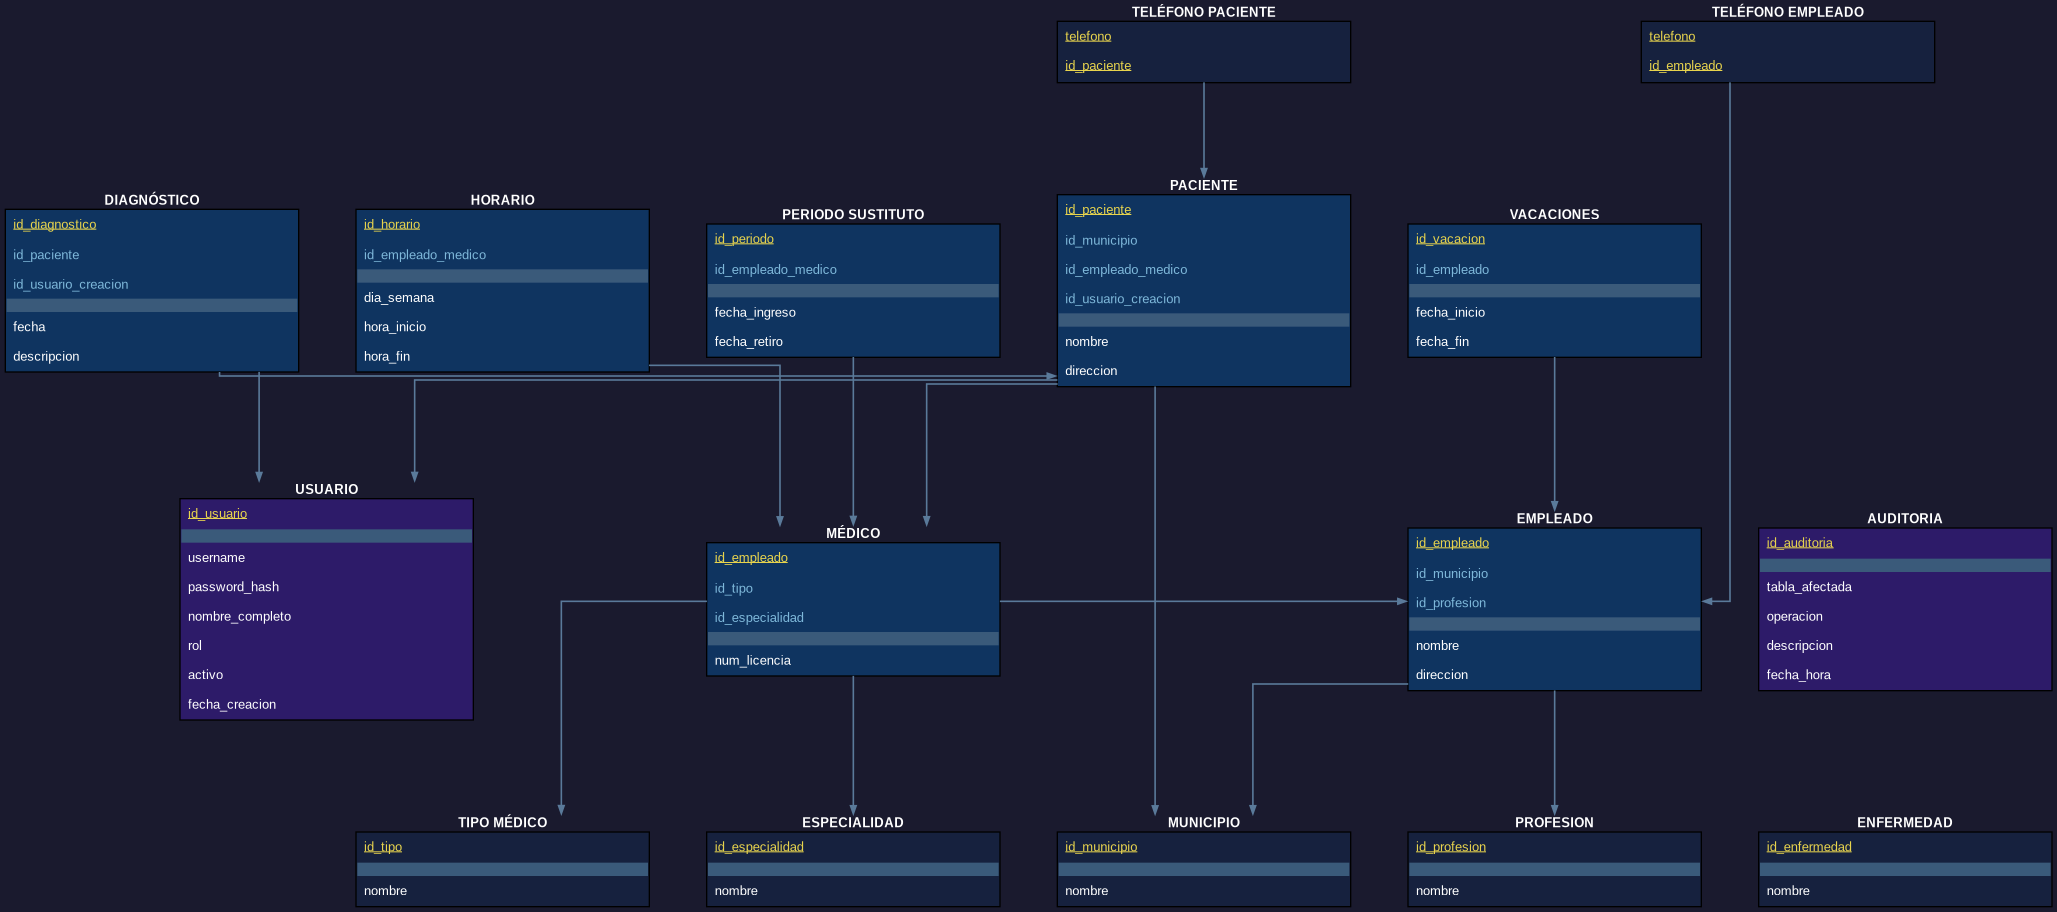
\includegraphics[width=1.0\textwidth]{Diagrama_Relacional_Normalizado.png}
    \caption{Diagrama del Modelo Relacional F\'isico y Normalizado}
    \label{fig:diagrama_relacional}
\end{figure}

Aspectos destacados del dise\~no relacional:

\begin{itemize}
    \item \textbf{Sin cruces en las l\'ineas:} Las conexiones entre tablas se redibujaron para que no se crucen, as\'i se ve m\'as claro.

    \item \textbf{Cardinalidad:} En las conexiones se puede ver cu\'antos registros de una tabla se relacionan con cu\'antos de la otra. Por ejemplo, un empleado puede tener varias vacaciones.

    \item \textbf{Sin PK ni FK en los nombres:} Los nombres de las columnas no traen ``PK'' o ``FK'' como nos hab\'ian dicho que no pus\'ieramos.

    \item \textbf{Normalizaci\'on:} Para que los tel\'efonos est\'en separados (porque pueden tener varios), se crearon tablas aparte: TELEFONO\_EMPLEADO y TELEFONO\_PACIENTE. Lo mismo con municipio, especialidad, profesi\'on y tipo de m\'edico, que son tablas de referencia para no repetir datos.
\end{itemize}

% ======================================================================
% SECCIÓN 4: DICCIONARIO DE DATOS
% ======================================================================
\newpage
\section{Diccionario de Datos}

Aqu\'i est\'a el diccionario de datos de la base de datos. Tiene todas las tablas, sus columnas, tipos de datos, restricciones y una breve descripci\'on de cada cosa.

\subsection{Descripci\'on de tablas y columnas}

\subsubsection{MUNICIPIO}
Almacena los municipios donde viven tanto los empleados como los pacientes del centro de salud.

{\small\begin{longtable}{|p{2.3cm}|p{3.3cm}|p{4.2cm}|p{4.2cm}|}
\hline
\textbf{Columna} & \textbf{Tipo} & \textbf{Restricciones} & \textbf{Descripci\'on} \\ \hline
\endfirsthead
\hline
\textbf{Columna} & \textbf{Tipo} & \textbf{Restricciones} & \textbf{Descripci\'on} \\ \hline
\endhead
id\_municipio & INT & PK, NOT NULL, AUTO\_INCREMENT & Identificador \'unico de cada municipio \\ \hline
nombre & VARCHAR(100) & NOT NULL & Nombre del municipio \\ \hline
\caption{MUNICIPIO}
\end{longtable}}

\subsubsection{ESPECIALIDAD}
Cat\'alogo de las especialidades m\'edicas que ofrece el centro de salud.

{\small\begin{longtable}{|p{2.3cm}|p{3.3cm}|p{4.2cm}|p{4.2cm}|}
\hline
\textbf{Columna} & \textbf{Tipo} & \textbf{Restricciones} & \textbf{Descripci\'on} \\ \hline
\endfirsthead
\hline
\textbf{Columna} & \textbf{Tipo} & \textbf{Restricciones} & \textbf{Descripci\'on} \\ \hline
\endhead
id\_especialidad & INT & PK, NOT NULL, AUTO\_INCREMENT & Identificador \'unico de la especialidad \\ \hline
nombre & VARCHAR(100) & NOT NULL & Nombre de la especialidad m\'edica \\ \hline
\caption{ESPECIALIDAD}
\end{longtable}}

\subsubsection{TIPO\_MEDICO}
Clasificaci\'on de los m\'edicos seg\'un su tipo de vinculaci\'on con el centro de salud.

{\small\begin{longtable}{|p{2.3cm}|p{3.3cm}|p{4.2cm}|p{4.2cm}|}
\hline
\textbf{Columna} & \textbf{Tipo} & \textbf{Restricciones} & \textbf{Descripci\'on} \\ \hline
\endfirsthead
\hline
\textbf{Columna} & \textbf{Tipo} & \textbf{Restricciones} & \textbf{Descripci\'on} \\ \hline
\endhead
id\_tipo & INT & PK, NOT NULL, AUTO\_INCREMENT & Identificador \'unico del tipo de m\'edico \\ \hline
nombre & VARCHAR(50) & NOT NULL & Nombre del tipo (Titular, Interino, Sustituto) \\ \hline
\caption{TIPO\_MEDICO}
\end{longtable}}

\subsubsection{PROFESION}
Cat\'alogo de las profesiones del personal no m\'edico que trabaja en el centro de salud.

{\small\begin{longtable}{|p{2.3cm}|p{3.3cm}|p{4.2cm}|p{4.2cm}|}
\hline
\textbf{Columna} & \textbf{Tipo} & \textbf{Restricciones} & \textbf{Descripci\'on} \\ \hline
\endfirsthead
\hline
\textbf{Columna} & \textbf{Tipo} & \textbf{Restricciones} & \textbf{Descripci\'on} \\ \hline
\endhead
id\_profesion & INT & PK, NOT NULL, AUTO\_INCREMENT & Identificador \'unico de la profesi\'on \\ \hline
nombre & VARCHAR(100) & NOT NULL & Nombre de la profesi\'on (Auxiliar, Vigilante, Administrativo) \\ \hline
\caption{PROFESION}
\end{longtable}}

\subsubsection{EMPLEADO}
Registro de todo el personal que trabaja en el centro de salud, incluyendo tanto a los m\'edicos como a los dem\'as empleados. Esta tabla contiene los datos b\'asicos que comparten todos los trabajadores.

{\small\begin{longtable}{|p{2.3cm}|p{3.3cm}|p{4.2cm}|p{4.2cm}|}
\hline
\textbf{Columna} & \textbf{Tipo} & \textbf{Restricciones} & \textbf{Descripci\'on} \\ \hline
\endfirsthead
\hline
\textbf{Columna} & \textbf{Tipo} & \textbf{Restricciones} & \textbf{Descripci\'on} \\ \hline
\endhead
id\_empleado & INT & PK, NOT NULL, AUTO\_INCREMENT & Identificador \'unico de cada empleado \\ \hline
id\_municipio & INT & FK $\rightarrow$ MUNICIPIO, NOT NULL & Municipio donde vive el empleado \\ \hline
id\_profesion & INT & FK $\rightarrow$ PROFESION, NULLABLE & Profesi\'on del empleado (puede ser nulo si es m\'edico) \\ \hline
nombre & VARCHAR(120) & NOT NULL & Nombre completo del empleado \\ \hline
direccion & VARCHAR(160) & NOT NULL & Direcci\'on de residencia del empleado \\ \hline
\caption{EMPLEADO}
\end{longtable}}

\subsubsection{MEDICO}
Informaci\'on adicional espec\'ifica de los m\'edicos. Esta tabla complementa los datos que ya est\'an en la tabla EMPLEADO, agregando la informaci\'on que solo aplica para el personal m\'edico.

{\small\begin{longtable}{|p{2.3cm}|p{3.3cm}|p{4.2cm}|p{4.2cm}|}
\hline
\textbf{Columna} & \textbf{Tipo} & \textbf{Restricciones} & \textbf{Descripci\'on} \\ \hline
\endfirsthead
\hline
\textbf{Columna} & \textbf{Tipo} & \textbf{Restricciones} & \textbf{Descripci\'on} \\ \hline
\endhead
id\_empleado & INT & PK, FK $\rightarrow$ EMPLEADO, NOT NULL & Identificador del m\'edico (mismo que en EMPLEADO) \\ \hline
num\_licencia & VARCHAR(50) & UNIQUE, NOT NULL & N\'umero de licencia m\'edica profesional \\ \hline
id\_tipo & INT & FK $\rightarrow$ TIPO\_MEDICO, NOT NULL & Tipo de vinculaci\'on del m\'edico \\ \hline
id\_especialidad & INT & FK $\rightarrow$ ESPECIALIDAD, NOT NULL & Especialidad m\'edica del doctor \\ \hline
\caption{MEDICO}
\end{longtable}}

\subsubsection{PACIENTE}
Registro de los pacientes que reciben atenci\'on en el centro de salud. Cada paciente queda asociado a un m\'edico responsable.

{\small\begin{longtable}{|p{2.3cm}|p{3.3cm}|p{4.2cm}|p{4.2cm}|}
\hline
\textbf{Columna} & \textbf{Tipo} & \textbf{Restricciones} & \textbf{Descripci\'on} \\ \hline
\endfirsthead
\hline
\textbf{Columna} & \textbf{Tipo} & \textbf{Restricciones} & \textbf{Descripci\'on} \\ \hline
\endhead
id\_paciente & INT & PK, NOT NULL, AUTO\_INCREMENT & Identificador \'unico de cada paciente \\ \hline
id\_municipio & INT & FK $\rightarrow$ MUNICIPIO, NOT NULL & Municipio donde vive el paciente \\ \hline
id\_empleado\_medico & INT & FK $\rightarrow$ MEDICO(id\_empleado), NOT NULL & M\'edico responsable del paciente \\ \hline
id\_usuario\_creacion & INT & FK $\rightarrow$ USUARIO, NULL, DEFAULT NULL & Usuario que registr\'o al paciente en el sistema \\ \hline
nombre & VARCHAR(120) & NOT NULL & Nombre completo del paciente \\ \hline
direccion & VARCHAR(160) & NOT NULL & Direcci\'on de residencia del paciente \\ \hline
\caption{PACIENTE}
\end{longtable}}

\textbf{Justificaci\'on de la FK:} La llave for\'anea del paciente debe apuntar a la tabla MEDICO y no directamente a EMPLEADO, porque el m\'edico responsable debe pertenecer al personal m\'edico del centro de salud. Esta restricci\'on evita que un paciente sea asignado por error a un auxiliar, vigilante o administrativo.

\subsubsection{HORARIO}
Registra los horarios de consulta de cada m\'edico, permitiendo que un m\'edico tenga horarios diferentes seg\'un el d\'ia de la semana.

{\small\begin{longtable}{|p{2.3cm}|p{3.3cm}|p{4.2cm}|p{4.2cm}|}
\hline
\textbf{Columna} & \textbf{Tipo} & \textbf{Restricciones} & \textbf{Descripci\'on} \\ \hline
\endfirsthead
\hline
\textbf{Columna} & \textbf{Tipo} & \textbf{Restricciones} & \textbf{Descripci\'on} \\ \hline
\endhead
id\_horario & INT & PK, NOT NULL, AUTO\_INCREMENT & Identificador \'unico del horario \\ \hline
id\_empleado\_medico & INT & FK $\rightarrow$ EMPLEADO, NOT NULL & M\'edico al que pertenece el horario \\ \hline
dia\_semana & ENUM('Lunes','Martes','Mi\'ercoles','Jueves','Viernes','S\'abado','Domingo') & NOT NULL & D\'ia de la semana del turno \\ \hline
hora\_inicio & TIME & NOT NULL & Hora a la que empieza el turno \\ \hline
hora\_fin & TIME & NOT NULL & Hora a la que termina el turno \\ \hline
\caption{HORARIO}
\end{longtable}}

\subsubsection{PERIODO\_SUSTITUTO}
Guarda el historial de todas las sustituciones que ha realizado cada m\'edico sustituto, con las fechas de ingreso y retiro.

{\small\begin{longtable}{|p{2.3cm}|p{3.3cm}|p{4.2cm}|p{4.2cm}|}
\hline
\textbf{Columna} & \textbf{Tipo} & \textbf{Restricciones} & \textbf{Descripci\'on} \\ \hline
\endfirsthead
\hline
\textbf{Columna} & \textbf{Tipo} & \textbf{Restricciones} & \textbf{Descripci\'on} \\ \hline
\endhead
id\_periodo & INT & PK, NOT NULL, AUTO\_INCREMENT & Identificador \'unico del periodo de sustituci\'on \\ \hline
id\_empleado\_medico & INT & FK $\rightarrow$ EMPLEADO, NOT NULL & M\'edico sustituto asociado \\ \hline
fecha\_ingreso & DATE & NOT NULL & Fecha en que empez\'o la sustituci\'on \\ \hline
fecha\_retiro & DATE & NULLABLE & Fecha en que termin\'o la sustituci\'on (puede estar vac\'ia si a\'un sigue activo) \\ \hline
\caption{PERIODO\_SUSTITUTO}
\end{longtable}}

\subsubsection{VACACIONES}
Almacena los periodos vacacionales de todos los trabajadores del centro, tanto m\'edicos como empleados. Esta tabla no tiene un campo para el estado; en lugar de eso, el estado se calcula comparando las fechas con la fecha actual.

{\small\begin{longtable}{|p{2.3cm}|p{3.3cm}|p{4.2cm}|p{4.2cm}|}
\hline
\textbf{Columna} & \textbf{Tipo} & \textbf{Restricciones} & \textbf{Descripci\'on} \\ \hline
\endfirsthead
\hline
\textbf{Columna} & \textbf{Tipo} & \textbf{Restricciones} & \textbf{Descripci\'on} \\ \hline
\endhead
id\_vacacion & INT & PK, NOT NULL, AUTO\_INCREMENT & Identificador \'unico del periodo vacacional \\ \hline
id\_empleado & INT & FK $\rightarrow$ EMPLEADO, NOT NULL & Empleado que solicita las vacaciones \\ \hline
fecha\_inicio & DATE & NOT NULL & Fecha en que empiezan las vacaciones \\ \hline
fecha\_fin & DATE & NOT NULL & Fecha en que terminan las vacaciones \\ \hline
\caption{VACACIONES}
\end{longtable}}

\subsubsection{USUARIO}
Almacena las cuentas de usuario del sistema con sus roles y contrase\~nas hasheadas. Esta tabla permite el inicio de sesi\'on en la aplicaci\'on y el control de acceso basado en roles (admin, m\'edico, enfermero, recepcionista).

{\small\begin{longtable}{|p{2.3cm}|p{3.3cm}|p{4.2cm}|p{4.2cm}|}
\hline
\textbf{Columna} & \textbf{Tipo} & \textbf{Restricciones} & \textbf{Descripci\'on} \\ \hline
\endfirsthead
\hline
\textbf{Columna} & \textbf{Tipo} & \textbf{Restricciones} & \textbf{Descripci\'on} \\ \hline
\endhead
id\_usuario & INT & PK, NOT NULL, AUTO\_INCREMENT & Identificador \'unico del usuario \\ \hline
username & VARCHAR(50) & NOT NULL, UNIQUE & Nombre de usuario para el inicio de sesi\'on \\ \hline
password\_hash & VARCHAR(255) & NOT NULL & Hash SHA-256 de la contrase\~na \\ \hline
nombre\_completo & VARCHAR(120) & NOT NULL & Nombre real del usuario \\ \hline
rol & ENUM('admin','medico','enfermero','recepcionista') & NOT NULL, DEFAULT 'medico' & Rol que determina los permisos en el sistema \\ \hline
activo & BOOLEAN & NOT NULL, DEFAULT TRUE & Indica si la cuenta est\'a activa \\ \hline
fecha\_creacion & DATETIME & DEFAULT CURRENT\_TIMESTAMP & Fecha de creaci\'on de la cuenta \\ \hline
\caption{USUARIO}
\end{longtable}}

\subsubsection{DIAGNOSTICO}
Registra los diagn\'osticos m\'edicos que se le han hecho a cada paciente a lo largo del tiempo, formando su historial cl\'inico. Cada diagn\'ostico registra tambi\'en el usuario que lo cre\'o.

{\small\begin{longtable}{|p{2.3cm}|p{3.3cm}|p{4.2cm}|p{4.2cm}|}
\hline
\textbf{Columna} & \textbf{Tipo} & \textbf{Restricciones} & \textbf{Descripci\'on} \\ \hline
\endfirsthead
\hline
\textbf{Columna} & \textbf{Tipo} & \textbf{Restricciones} & \textbf{Descripci\'on} \\ \hline
\endhead
id\_diagnostico & INT & PK, NOT NULL, AUTO\_INCREMENT & Identificador \'unico del diagn\'ostico \\ \hline
id\_paciente & INT & FK $\rightarrow$ PACIENTE, NOT NULL & Paciente al que pertenece el diagn\'ostico \\ \hline
id\_usuario\_creacion & INT & FK $\rightarrow$ USUARIO, NULL, DEFAULT NULL & Usuario que registr\'o el diagn\'ostico \\ \hline
fecha & DATE & NOT NULL & Fecha en que se hizo el diagn\'ostico \\ \hline
descripcion & VARCHAR(255) & NOT NULL & Descripci\'on detallada del diagn\'ostico \\ \hline
\caption{DIAGNOSTICO}
\end{longtable}}

\subsubsection{TELEFONO\_EMPLEADO}
Permite registrar varios n\'umeros de tel\'efono para cada empleado, ya que una persona puede tener m\'as de un medio de contacto.

{\small\begin{longtable}{|p{2.3cm}|p{3.3cm}|p{4.2cm}|p{4.2cm}|}
\hline
\textbf{Columna} & \textbf{Tipo} & \textbf{Restricciones} & \textbf{Descripci\'on} \\ \hline
\endfirsthead
\hline
\textbf{Columna} & \textbf{Tipo} & \textbf{Restricciones} & \textbf{Descripci\'on} \\ \hline
\endhead
id\_empleado & INT & PK, FK $\rightarrow$ EMPLEADO, NOT NULL & Empleado al que pertenece el tel\'efono \\ \hline
telefono & VARCHAR(20) & PK, NOT NULL & N\'umero de tel\'efono del empleado \\ \hline
\caption{TELEFONO\_EMPLEADO}
\end{longtable}}

\subsubsection{TELEFONO\_PACIENTE}
Permite registrar varios n\'umeros de tel\'efono para cada paciente, de manera similar a como se hace con los empleados.

{\small\begin{longtable}{|p{2.3cm}|p{3.3cm}|p{4.2cm}|p{4.2cm}|}
\hline
\textbf{Columna} & \textbf{Tipo} & \textbf{Restricciones} & \textbf{Descripci\'on} \\ \hline
\endfirsthead
\hline
\textbf{Columna} & \textbf{Tipo} & \textbf{Restricciones} & \textbf{Descripci\'on} \\ \hline
\endhead
id\_paciente & INT & PK, FK $\rightarrow$ PACIENTE, NOT NULL & Paciente al que pertenece el tel\'efono \\ \hline
telefono & VARCHAR(20) & PK, NOT NULL & N\'umero de tel\'efono del paciente \\ \hline
\caption{TELEFONO\_PACIENTE}
\end{longtable}}

\newpage

\subsection{Vistas}

\subsubsection{vw\_pacientes\_medicos}
Muestra cada paciente junto con el m\'edico responsable que tiene asignado, incluyendo la especialidad y tipo de cada m\'edico. Se usa para el reporte de pacientes por especialidad.

{\small\begin{longtable}{|p{2.3cm}|p{3.3cm}|p{8cm}|}
\hline
\textbf{Columna} & \textbf{Tipo} & \textbf{Descripci\'on} \\ \hline
\endfirsthead
\hline
\textbf{Columna} & \textbf{Tipo} & \textbf{Descripci\'on} \\ \hline
\endhead
id\_paciente & INT & Identificador del paciente \\ \hline
paciente & VARCHAR(120) & Nombre completo del paciente \\ \hline
direccion\_paciente & VARCHAR(160) & Direcci\'on del paciente \\ \hline
municipio\_paciente & VARCHAR(100) & Municipio de residencia del paciente \\ \hline
id\_medico & INT & Identificador del m\'edico \\ \hline
medico & VARCHAR(120) & Nombre completo del m\'edico \\ \hline
num\_licencia & VARCHAR(50) & N\'umero de licencia m\'edica \\ \hline
especialidad & VARCHAR(100) & Especialidad del m\'edico \\ \hline
tipo\_medico & VARCHAR(50) & Tipo de vinculaci\'on del m\'edico \\ \hline
\caption{vw\_pacientes\_medicos}
\end{longtable}}

\subsubsection{vw\_medicos\_info}
Proporciona la informaci\'on detallada de todos los m\'edicos registrados: datos personales, licencia, tipo y especialidad. Es la vista principal para el directorio m\'edico.

{\small\begin{longtable}{|p{2.3cm}|p{3.3cm}|p{8cm}|}
\hline
\textbf{Columna} & \textbf{Tipo} & \textbf{Descripci\'on} \\ \hline
\endfirsthead
\hline
\textbf{Columna} & \textbf{Tipo} & \textbf{Descripci\'on} \\ \hline
\endhead
id\_medico & INT & Identificador del m\'edico \\ \hline
medico & VARCHAR(120) & Nombre completo del m\'edico \\ \hline
direccion & VARCHAR(160) & Direcci\'on de residencia \\ \hline
municipio & VARCHAR(100) & Municipio donde vive \\ \hline
num\_licencia & VARCHAR(50) & N\'umero de licencia m\'edica \\ \hline
tipo\_medico & VARCHAR(50) & Tipo de vinculaci\'on \\ \hline
especialidad & VARCHAR(100) & Especialidad m\'edica \\ \hline
\caption{vw\_medicos\_info}
\end{longtable}}

\subsubsection{vw\_diagnosticos\_pacientes}
Consolida los diagn\'osticos m\'edicos con los datos del paciente y su m\'edico tratante. Permite buscar pacientes por enfermedad para el reporte correspondiente.

{\small\begin{longtable}{|p{2.3cm}|p{3.3cm}|p{8cm}|}
\hline
\textbf{Columna} & \textbf{Tipo} & \textbf{Descripci\'on} \\ \hline
\endfirsthead
\hline
\textbf{Columna} & \textbf{Tipo} & \textbf{Descripci\'on} \\ \hline
\endhead
id\_diagnostico & INT & Identificador del diagn\'ostico \\ \hline
fecha & DATE & Fecha del diagn\'ostico \\ \hline
diagnostico & VARCHAR(255) & Descripci\'on del diagn\'ostico \\ \hline
id\_paciente & INT & Identificador del paciente \\ \hline
paciente & VARCHAR(120) & Nombre del paciente \\ \hline
direccion\_paciente & VARCHAR(160) & Direcci\'on del paciente \\ \hline
municipio\_paciente & VARCHAR(100) & Municipio del paciente \\ \hline
id\_medico & INT & Identificador del m\'edico tratante \\ \hline
medico & VARCHAR(120) & Nombre del m\'edico tratante \\ \hline
especialidad & VARCHAR(100) & Especialidad del m\'edico \\ \hline
\caption{vw\_diagnosticos\_pacientes}
\end{longtable}}

\subsubsection{vw\_vacaciones\_medicos}
Lista los periodos vacacionales del personal m\'edico con el estado calculado autom\'aticamente (``Planeadas'', ``En curso'' o ``Disfrutadas'') seg\'un la fecha actual del sistema.

{\small\begin{longtable}{|p{2.3cm}|p{3.3cm}|p{8cm}|}
\hline
\textbf{Columna} & \textbf{Tipo} & \textbf{Descripci\'on} \\ \hline
\endfirsthead
\hline
\textbf{Columna} & \textbf{Tipo} & \textbf{Descripci\'on} \\ \hline
\endhead
id\_vacacion & INT & Identificador del periodo vacacional \\ \hline
fecha\_inicio & DATE & Fecha de inicio de las vacaciones \\ \hline
fecha\_fin & DATE & Fecha de fin de las vacaciones \\ \hline
id\_medico & INT & Identificador del m\'edico \\ \hline
medico & VARCHAR(120) & Nombre del m\'edico \\ \hline
especialidad & VARCHAR(100) & Especialidad del m\'edico \\ \hline
estado\_vacaciones & VARCHAR(20) & Estado calculado (Planeadas, En curso, Disfrutadas) \\ \hline
\caption{vw\_vacaciones\_medicos}
\end{longtable}}

\subsubsection{vw\_sustitutos\_estado}
Muestra el estado actual de los m\'edicos sustitutos a partir de su \'ultimo periodo de sustituci\'on registrado. Permite saber si el sustituto est\'a activo o inactivo sin eliminar su historial.

{\small\begin{longtable}{|p{2.3cm}|p{3.3cm}|p{8cm}|}
\hline
\textbf{Columna} & \textbf{Tipo} & \textbf{Descripci\'on} \\ \hline
\endfirsthead
\hline
\textbf{Columna} & \textbf{Tipo} & \textbf{Descripci\'on} \\ \hline
\endhead
id\_medico & INT & Identificador del m\'edico sustituto \\ \hline
medico & VARCHAR(120) & Nombre completo del m\'edico \\ \hline
ultima\_fecha\_ingreso & DATE & \'Ultima fecha de ingreso registrada \\ \hline
fecha\_retiro\_ultimo\_periodo & DATE & Fecha de retiro asociada al \'ultimo periodo \\ \hline
estado\_sustituto & VARCHAR(20) & Estado calculado: Activo o Inactivo \\ \hline
\caption{vw\_sustitutos\_estado}
\end{longtable}}

\newpage

\subsection{Procedimientos Almacenados}

Los procedimientos almacenados los usamos para generar los reportes que pide el enunciado. Reciben par\'ametros y devuelven los resultados directamente.

\subsubsection{sp\_pacientes\_por\_especialidad}
Recibe el nombre de una especialidad y devuelve todos los pacientes que est\'an a cargo de m\'edicos de esa especialidad. Internamente consulta la vista \texttt{vw\_pacientes\_medicos}.

{\small\begin{verbatim}
DELIMITER $$

DROP PROCEDURE IF EXISTS sp_pacientes_por_especialidad $$
CREATE PROCEDURE sp_pacientes_por_especialidad(IN p_especialidad VARCHAR(100))
BEGIN
    SELECT *
    FROM vw_pacientes_medicos
    WHERE especialidad = p_especialidad
    ORDER BY medico, paciente;
END $$

DELIMITER ;
\end{verbatim}}

\subsubsection{sp\_medicos\_disponibles\_por\_especialidad}
Dada una especialidad, lista los m\'edicos que est\'an disponibles actualmente (no est\'an de vacaciones ni son sustitutos inactivos), junto con sus horarios de consulta.

{\small\begin{verbatim}
DELIMITER $$

DROP PROCEDURE IF EXISTS sp_medicos_disponibles_por_especialidad $$
CREATE PROCEDURE sp_medicos_disponibles_por_especialidad(IN p_especialidad VARCHAR(100))
BEGIN
    SELECT
        mi.id_medico,
        mi.medico,
        mi.num_licencia,
        mi.tipo_medico,
        mi.especialidad,
        GROUP_CONCAT(CONCAT(h.dia_semana, ' ',
            TIME_FORMAT(h.hora_inicio, '%H:%i'), '-',
            TIME_FORMAT(h.hora_fin, '%H:%i'))
            ORDER BY FIELD(h.dia_semana, 'Lunes','Martes',
                'Miércoles','Jueves','Viernes','Sábado','Domingo')
            SEPARATOR ' | ') AS horarios
    FROM vw_medicos_info mi
    LEFT JOIN horario h ON mi.id_medico = h.id_empleado_medico
    WHERE mi.especialidad = p_especialidad
      AND NOT EXISTS (
          SELECT 1
          FROM vacaciones v
          WHERE v.id_empleado = mi.id_medico
            AND CURDATE() BETWEEN v.fecha_inicio AND v.fecha_fin
      )
      AND (
          mi.tipo_medico <> 'Sustituto'
          OR EXISTS (
              SELECT 1
              FROM periodo_sustituto ps
              WHERE ps.id_empleado_medico = mi.id_medico
                AND ps.fecha_ingreso = (
                    SELECT MAX(ps2.fecha_ingreso)
                    FROM periodo_sustituto ps2
                    WHERE ps2.id_empleado_medico = mi.id_medico
                )
                AND (ps.fecha_retiro IS NULL
                     OR ps.fecha_ingreso > ps.fecha_retiro
                     OR CURDATE() <= ps.fecha_retiro)
          )
      )
    GROUP BY mi.id_medico, mi.medico, mi.num_licencia,
             mi.tipo_medico, mi.especialidad
    ORDER BY mi.medico;
END $$

DELIMITER ;
\end{verbatim}}

\subsubsection{sp\_pacientes\_por\_diagnostico}
Busca pacientes cuyo diagn\'ostico contenga una palabra clave (por ejemplo, ``Hipertensi\'on'' o ``Diabetes''). Devuelve los resultados ordenados del m\'as reciente al m\'as antiguo.

{\small\begin{verbatim}
DELIMITER $$

DROP PROCEDURE IF EXISTS sp_pacientes_por_diagnostico $$
CREATE PROCEDURE sp_pacientes_por_diagnostico(IN p_busqueda VARCHAR(100))
BEGIN
    SELECT *
    FROM vw_diagnosticos_pacientes
    WHERE diagnostico LIKE CONCAT('%', p_busqueda, '%')
    ORDER BY fecha DESC, paciente;
END $$

DELIMITER ;
\end{verbatim}}

\subsubsection{sp\_vacaciones\_medicos\_intervalo}
Devuelve los m\'edicos que tienen vacaciones programadas dentro de un rango de fechas espec\'ifico. \'Util para consultar la disponibilidad del personal en un periodo determinado.

{\small\begin{verbatim}
DELIMITER $$

DROP PROCEDURE IF EXISTS sp_vacaciones_medicos_intervalo $$
CREATE PROCEDURE sp_vacaciones_medicos_intervalo(
    IN p_fecha_inicio DATE,
    IN p_fecha_fin DATE
)
BEGIN
    SELECT *
    FROM vw_vacaciones_medicos
    WHERE fecha_inicio <= p_fecha_fin
      AND fecha_fin >= p_fecha_inicio
    ORDER BY fecha_inicio, medico;
END $$

DELIMITER ;
\end{verbatim}}

\newpage

\subsection{Triggers}

Los disparadores (triggers) se implementan para reforzar reglas de negocio que no pueden garantizarse completamente mediante claves primarias, llaves foráneas o restricciones CHECK simples. Estos triggers permiten validar automáticamente la información antes de insertar o actualizar registros en tablas críticas del sistema.

Con estos triggers, la base de datos no depende únicamente de la aplicación para proteger la integridad de la información. Si alguien intenta insertar datos inconsistentes desde MySQL Workbench, desde la aplicación o desde cualquier otra herramienta, el motor de base de datos rechazará la operación y mostrará un mensaje de error.

{\small\begin{longtable}{|p{3.5cm}|p{2cm}|p{2cm}|p{1.5cm}|p{6cm}|}
\hline
\textbf{Trigger} & \textbf{Tabla} & \textbf{Momento} & \textbf{Evento} & \textbf{Regla que valida} \\ \hline
\endfirsthead
\hline
\textbf{Trigger} & \textbf{Tabla} & \textbf{Momento} & \textbf{Evento} & \textbf{Regla que valida} \\ \hline
\endhead

trg\_horario\_no\_traslape\_bi & horario & BEFORE & INSERT & Evita que un médico tenga horarios que se crucen el mismo día \\ \hline
trg\_horario\_no\_traslape\_bu & horario & BEFORE & UPDATE & Evita que una actualización genere cruces de horarios \\ \hline
trg\_vacaciones\_no\_traslape\_bi & vacaciones & BEFORE & INSERT & Evita que un empleado tenga vacaciones cruzadas \\ \hline
trg\_vacaciones\_no\_traslape\_bu & vacaciones & BEFORE & UPDATE & Evita que una actualización genere vacaciones superpuestas \\ \hline
trg\_periodo\_sustituto\_valida\_bi & periodo\_sustituto & BEFORE & INSERT & Solo los médicos de tipo Sustituto pueden tener periodos de sustitución; además evita traslapes \\ \hline
trg\_periodo\_sustituto\_valida\_bu & periodo\_sustituto & BEFORE & UPDATE & Valida cambios en periodos de sustitución \\ \hline
trg\_diagnostico\_valida\_bi & diagnostico & BEFORE & INSERT & Evita diagnósticos con fecha futura o descripción demasiado corta \\ \hline
trg\_diagnostico\_valida\_bu & diagnostico & BEFORE & UPDATE & Valida cambios en diagnósticos existentes \\ \hline
trg\_paciente\_medico\_disponible\_bi & paciente & BEFORE & INSERT & Evita asignar pacientes a médicos que están de vacaciones o son sustitutos inactivos \\ \hline
trg\_paciente\_medico\_disponible\_bu & paciente & BEFORE & UPDATE & Valida el cambio de médico responsable \\ \hline
trg\_medico\_empleado\_profesion\_bi & medico & BEFORE & INSERT & Evita registrar como médico a un empleado que tenga profesión no médica \\ \hline
trg\_auditoria\_paciente\_ai & paciente & AFTER & INSERT & Registra en la bitácora (auditoria) cuando se crea un paciente \\ \hline
trg\_auditoria\_diagnostico\_ai & diagnostico & AFTER & INSERT & Registra en la bitácora cuando se crea un diagnóstico \\ \hline
trg\_auditoria\_vacaciones\_ai & vacaciones & AFTER & INSERT & Registra en la bitácora cuando se registran vacaciones \\ \hline
\caption{Triggers implementados en la base de datos}
\end{longtable}}

% ======================================================================
% SECCIÓN 5: CÓDIGO FUENTE
% ======================================================================
\newpage
\section{C\'odigo Fuente}

En esta secci\'on se incluye el c\'odigo fuente utilizado para crear la base de datos y conectar la aplicaci\'on con ella. Todo el c\'odigo est\'a escrito para MySQL.

\subsection{Estructura de la Base de Datos (DDL)}

Aqu\'i van los comandos para crear la base de datos y sus tablas. Tiene restricciones como claves for\'aneas con \texttt{ON DELETE CASCADE}, \texttt{CHECK} y \texttt{UNIQUE} para no duplicar datos. Primero las tablas param\'etricas (las de referencia como municipios y especialidades), luego las principales y al final las de tel\'efonos.

{\small\begin{verbatim}
DROP DATABASE IF EXISTS centro_salud;
CREATE DATABASE centro_salud
  CHARACTER SET utf8mb4
  COLLATE utf8mb4_unicode_ci;

USE centro_salud;

CREATE TABLE municipio (
    id_municipio INT AUTO_INCREMENT PRIMARY KEY,
    nombre VARCHAR(100) NOT NULL UNIQUE
) ENGINE=InnoDB;

CREATE TABLE profesion (
    id_profesion INT AUTO_INCREMENT PRIMARY KEY,
    nombre VARCHAR(100) NOT NULL UNIQUE
) ENGINE=InnoDB;

CREATE TABLE especialidad (
    id_especialidad INT AUTO_INCREMENT PRIMARY KEY,
    nombre VARCHAR(100) NOT NULL UNIQUE
) ENGINE=InnoDB;

CREATE TABLE tipo_medico (
    id_tipo INT AUTO_INCREMENT PRIMARY KEY,
    nombre VARCHAR(50) NOT NULL UNIQUE
) ENGINE=InnoDB;

CREATE TABLE empleado (
    id_empleado INT AUTO_INCREMENT PRIMARY KEY,
    id_municipio INT NOT NULL,
    id_profesion INT NULL,
    nombre VARCHAR(120) NOT NULL,
    direccion VARCHAR(160) NOT NULL,
    CONSTRAINT fk_empleado_municipio
        FOREIGN KEY (id_municipio) REFERENCES municipio(id_municipio),
    CONSTRAINT fk_empleado_profesion
        FOREIGN KEY (id_profesion) REFERENCES profesion(id_profesion)
) ENGINE=InnoDB;

CREATE TABLE medico (
    id_empleado INT PRIMARY KEY,
    num_licencia VARCHAR(50) NOT NULL UNIQUE,
    id_tipo INT NOT NULL,
    id_especialidad INT NOT NULL,
    CONSTRAINT fk_medico_empleado
        FOREIGN KEY (id_empleado) REFERENCES empleado(id_empleado)
        ON DELETE CASCADE,
    CONSTRAINT fk_medico_tipo
        FOREIGN KEY (id_tipo) REFERENCES tipo_medico(id_tipo),
    CONSTRAINT fk_medico_especialidad
        FOREIGN KEY (id_especialidad) REFERENCES especialidad(id_especialidad)
) ENGINE=InnoDB;

CREATE TABLE telefono_empleado (
    id_empleado INT NOT NULL,
    telefono VARCHAR(20) NOT NULL,
    PRIMARY KEY (id_empleado, telefono),
    CONSTRAINT fk_tel_empleado
        FOREIGN KEY (id_empleado) REFERENCES empleado(id_empleado)
        ON DELETE CASCADE
) ENGINE=InnoDB;

CREATE TABLE horario (
    id_horario INT AUTO_INCREMENT PRIMARY KEY,
    id_empleado_medico INT NOT NULL,
    dia_semana ENUM('Lunes','Martes','Miercoles','Jueves',
                    'Viernes','Sabado','Domingo') NOT NULL,
    hora_inicio TIME NOT NULL,
    hora_fin TIME NOT NULL,
    CONSTRAINT fk_horario_medico
        FOREIGN KEY (id_empleado_medico) REFERENCES medico(id_empleado)
        ON DELETE CASCADE,
    CONSTRAINT chk_horario_horas
        CHECK (hora_fin > hora_inicio),
    CONSTRAINT uq_horario_medico_dia_hora
        UNIQUE (id_empleado_medico, dia_semana, hora_inicio, hora_fin)
) ENGINE=InnoDB;

CREATE TABLE periodo_sustituto (
    id_periodo INT AUTO_INCREMENT PRIMARY KEY,
    id_empleado_medico INT NOT NULL,
    fecha_ingreso DATE NOT NULL,
    fecha_retiro DATE NULL,
    CONSTRAINT fk_periodo_sustituto_medico
        FOREIGN KEY (id_empleado_medico) REFERENCES medico(id_empleado)
        ON DELETE CASCADE,
    CONSTRAINT chk_periodo_fechas
        CHECK (fecha_retiro IS NULL OR fecha_retiro >= fecha_ingreso)
) ENGINE=InnoDB;

CREATE TABLE vacaciones (
    id_vacacion INT AUTO_INCREMENT PRIMARY KEY,
    id_empleado INT NOT NULL,
    fecha_inicio DATE NOT NULL,
    fecha_fin DATE NOT NULL,
    CONSTRAINT fk_vacaciones_empleado
        FOREIGN KEY (id_empleado) REFERENCES empleado(id_empleado)
        ON DELETE CASCADE,
    CONSTRAINT chk_vacaciones_fechas
        CHECK (fecha_fin >= fecha_inicio)
) ENGINE=InnoDB;

CREATE TABLE paciente (
    id_paciente INT AUTO_INCREMENT PRIMARY KEY,
    id_municipio INT NOT NULL,
    id_empleado_medico INT NOT NULL,
    nombre VARCHAR(120) NOT NULL,
    direccion VARCHAR(160) NOT NULL,
    CONSTRAINT fk_paciente_municipio
        FOREIGN KEY (id_municipio) REFERENCES municipio(id_municipio),
    CONSTRAINT fk_paciente_medico
        FOREIGN KEY (id_empleado_medico) REFERENCES medico(id_empleado)
) ENGINE=InnoDB;

CREATE TABLE telefono_paciente (
    id_paciente INT NOT NULL,
    telefono VARCHAR(20) NOT NULL,
    PRIMARY KEY (id_paciente, telefono),
    CONSTRAINT fk_tel_paciente
        FOREIGN KEY (id_paciente) REFERENCES paciente(id_paciente)
        ON DELETE CASCADE
) ENGINE=InnoDB;

CREATE TABLE diagnostico (
    id_diagnostico INT AUTO_INCREMENT PRIMARY KEY,
    id_paciente INT NOT NULL,
    fecha DATE NOT NULL,
    descripcion VARCHAR(255) NOT NULL,
    CONSTRAINT fk_diagnostico_paciente
        FOREIGN KEY (id_paciente) REFERENCES paciente(id_paciente)
        ON DELETE CASCADE
) ENGINE=InnoDB;

-- TABLA DE USUARIOS (autenticaci\'on y roles)

CREATE TABLE usuario (
    id_usuario INT AUTO_INCREMENT PRIMARY KEY,
    username VARCHAR(50) NOT NULL UNIQUE,
    password_hash VARCHAR(255) NOT NULL,
    nombre_completo VARCHAR(120) NOT NULL,
    rol ENUM('admin','medico','enfermero','recepcionista') NOT NULL DEFAULT 'medico',
    activo BOOLEAN NOT NULL DEFAULT TRUE,
    fecha_creacion DATETIME DEFAULT CURRENT_TIMESTAMP
) ENGINE=InnoDB;

-- TABLA DE ENFERMEDADES (cat\'alogo para selector en la app)

CREATE TABLE enfermedad (
    id_enfermedad INT AUTO_INCREMENT PRIMARY KEY,
    nombre VARCHAR(150) NOT NULL UNIQUE
) ENGINE=InnoDB;

-- MODIFICACIONES PARA CONTROL DE USUARIO
-- Se agrega el campo id_usuario_creacion a paciente y diagnostico
-- para registrar qui\'en realiz\'o cada operaci\'on en el sistema.

ALTER TABLE paciente
ADD COLUMN id_usuario_creacion INT DEFAULT NULL AFTER id_empleado_medico,
ADD CONSTRAINT fk_paciente_usuario
    FOREIGN KEY (id_usuario_creacion) REFERENCES usuario(id_usuario)
    ON DELETE SET NULL;

ALTER TABLE diagnostico
ADD COLUMN id_usuario_creacion INT DEFAULT NULL AFTER id_paciente,
ADD CONSTRAINT fk_diagnostico_usuario
    FOREIGN KEY (id_usuario_creacion) REFERENCES usuario(id_usuario)
    ON DELETE SET NULL;

-- VISTAS (las armamos para los reportes)

CREATE OR REPLACE VIEW vw_pacientes_medicos AS
SELECT
    p.id_paciente,
    p.nombre AS paciente,
    p.direccion AS direccion_paciente,
    mp.nombre AS municipio_paciente,
    em.id_empleado AS id_medico,
    em.nombre AS medico,
    med.num_licencia,
    esp.nombre AS especialidad,
    tm.nombre AS tipo_medico
FROM paciente p
JOIN municipio mp ON p.id_municipio = mp.id_municipio
JOIN medico med ON p.id_empleado_medico = med.id_empleado
JOIN empleado em ON med.id_empleado = em.id_empleado
JOIN especialidad esp ON med.id_especialidad = esp.id_especialidad
JOIN tipo_medico tm ON med.id_tipo = tm.id_tipo;

CREATE OR REPLACE VIEW vw_medicos_info AS
SELECT
    e.id_empleado AS id_medico,
    e.nombre AS medico,
    e.direccion,
    mu.nombre AS municipio,
    m.num_licencia,
    tm.nombre AS tipo_medico,
    esp.nombre AS especialidad
FROM medico m
JOIN empleado e ON m.id_empleado = e.id_empleado
JOIN municipio mu ON e.id_municipio = mu.id_municipio
JOIN tipo_medico tm ON m.id_tipo = tm.id_tipo
JOIN especialidad esp ON m.id_especialidad = esp.id_especialidad;

CREATE OR REPLACE VIEW vw_diagnosticos_pacientes AS
SELECT
    d.id_diagnostico,
    d.fecha,
    d.descripcion AS diagnostico,
    p.id_paciente,
    p.nombre AS paciente,
    p.direccion AS direccion_paciente,
    mp.nombre AS municipio_paciente,
    em.id_empleado AS id_medico,
    em.nombre AS medico,
    esp.nombre AS especialidad
FROM diagnostico d
JOIN paciente p ON d.id_paciente = p.id_paciente
JOIN municipio mp ON p.id_municipio = mp.id_municipio
JOIN medico med ON p.id_empleado_medico = med.id_empleado
JOIN empleado em ON med.id_empleado = em.id_empleado
JOIN especialidad esp ON med.id_especialidad = esp.id_especialidad;

CREATE OR REPLACE VIEW vw_vacaciones_medicos AS
SELECT
    v.id_vacacion,
    v.fecha_inicio,
    v.fecha_fin,
    e.id_empleado AS id_medico,
    e.nombre AS medico,
    esp.nombre AS especialidad,
    CASE
        WHEN CURDATE() > v.fecha_fin THEN 'Disfrutadas'
        WHEN CURDATE() BETWEEN v.fecha_inicio AND v.fecha_fin THEN 'En curso'
        ELSE 'Planeadas'
    END AS estado_vacaciones
FROM vacaciones v
JOIN medico m ON v.id_empleado = m.id_empleado
JOIN empleado e ON m.id_empleado = e.id_empleado
JOIN especialidad esp ON m.id_especialidad = esp.id_especialidad;

CREATE OR REPLACE VIEW vw_usuarios_activos AS
SELECT
    u.id_usuario,
    u.username,
    u.password_hash,
    u.nombre_completo,
    u.rol
FROM usuario u
WHERE u.activo = TRUE;

-- PROCEDIMIENTOS ALMACENADOS
-- (para los reportes del enunciado)

DELIMITER $$

DROP PROCEDURE IF EXISTS sp_pacientes_por_especialidad $$
CREATE PROCEDURE sp_pacientes_por_especialidad(IN p_especialidad VARCHAR(100))
BEGIN
    SELECT *
    FROM vw_pacientes_medicos
    WHERE especialidad = p_especialidad
    ORDER BY medico, paciente;
END $$

DROP PROCEDURE IF EXISTS sp_medicos_disponibles_por_especialidad $$
CREATE PROCEDURE sp_medicos_disponibles_por_especialidad(IN p_especialidad VARCHAR(100))
BEGIN
    SELECT
        mi.id_medico,
        mi.medico,
        mi.num_licencia,
        mi.tipo_medico,
        mi.especialidad,
        GROUP_CONCAT(CONCAT(h.dia_semana, ' ',
            TIME_FORMAT(h.hora_inicio, '%H:%i'), '-',
            TIME_FORMAT(h.hora_fin, '%H:%i'))
            ORDER BY FIELD(h.dia_semana, 'Lunes','Martes',
                'Miercoles','Jueves','Viernes','Sabado','Domingo')
            SEPARATOR ' | ') AS horarios
    FROM vw_medicos_info mi
    LEFT JOIN horario h ON mi.id_medico = h.id_empleado_medico
    WHERE mi.especialidad = p_especialidad
      AND NOT EXISTS (
          SELECT 1
          FROM vacaciones v
          WHERE v.id_empleado = mi.id_medico
            AND CURDATE() BETWEEN v.fecha_inicio AND v.fecha_fin
      )
      AND (
          mi.tipo_medico <> 'Sustituto'
          OR EXISTS (
              SELECT 1
              FROM periodo_sustituto ps
              WHERE ps.id_empleado_medico = mi.id_medico
                AND ps.fecha_ingreso = (
                    SELECT MAX(ps2.fecha_ingreso)
                    FROM periodo_sustituto ps2
                    WHERE ps2.id_empleado_medico = mi.id_medico
                )
                AND (ps.fecha_retiro IS NULL
                     OR ps.fecha_ingreso > ps.fecha_retiro
                     OR CURDATE() <= ps.fecha_retiro)
          )
      )
    GROUP BY mi.id_medico, mi.medico, mi.num_licencia,
             mi.tipo_medico, mi.especialidad
    ORDER BY mi.medico;
END $$

DROP PROCEDURE IF EXISTS sp_pacientes_por_diagnostico $$
CREATE PROCEDURE sp_pacientes_por_diagnostico(IN p_busqueda VARCHAR(100))
BEGIN
    SELECT *
    FROM vw_diagnosticos_pacientes
    WHERE diagnostico LIKE CONCAT('%', p_busqueda, '%')
    ORDER BY fecha DESC, paciente;
END $$

DROP PROCEDURE IF EXISTS sp_vacaciones_medicos_intervalo $$
CREATE PROCEDURE sp_vacaciones_medicos_intervalo(
    IN p_fecha_inicio DATE,
    IN p_fecha_fin DATE
)
BEGIN
    SELECT *
    FROM vw_vacaciones_medicos
    WHERE fecha_inicio <= p_fecha_fin
      AND fecha_fin >= p_fecha_inicio
    ORDER BY fecha_inicio, medico;
END $$

DELIMITER ;
\end{verbatim}}

\subsection{Inserci\'on de Datos (DML)}

Estos son los datos de prueba para poblar la base de datos y probar que todo funcione. Incluye municipios, especialidades, tipos de m\'edico, profesiones, empleados, m\'edicos, tel\'efonos, horarios, periodos de sustituci\'on, vacaciones, pacientes y diagn\'osticos.

{\small\begin{verbatim}
-- DATOS PARAMETRICOS

INSERT INTO municipio (nombre) VALUES
('Bogota'),
('Soacha'),
('Chia'),
('Facatativa'),
('Zipaquirá');

INSERT INTO profesion (nombre) VALUES
('Auxiliar de enfermeria'),
('Vigilante'),
('Administrativo');

INSERT INTO especialidad (nombre) VALUES
('Medicina General'),
('Pediatria'),
('Cardiologia'),
('Dermatologia'),
('Ginecologia');

INSERT INTO tipo_medico (nombre) VALUES
('Titular'),
('Interino'),
('Sustituto');

-- EMPLEADOS

INSERT INTO empleado (id_municipio, id_profesion, nombre, direccion) VALUES
(1, NULL, 'Ana Maria Torres', 'Cra 10 # 20-30'),
(1, NULL, 'Carlos Perez Gomez', 'Calle 45 # 12-80'),
(2, NULL, 'Laura Rodriguez Diaz', 'Av Siempre Viva # 123'),
(3, NULL, 'Miguel Angel Rojas', 'Cra 7 # 90-15'),
(4, NULL, 'Sofia Martinez Leon', 'Calle 8 # 5-22'),
(1, 1, 'Diana Carolina Ruiz', 'Calle 30 # 15-40'),
(2, 2, 'Jorge Eliecer Ramos', 'Cra 9 # 13-17'),
(1, 3, 'Patricia Moreno Silva', 'Av Caracas # 40-55');

-- MEDICOS (heredan de EMPLEADO)

INSERT INTO medico (id_empleado, num_licencia, id_tipo, id_especialidad) VALUES
(1, 'LIC-MG-001', 1, 1),
(2, 'LIC-PED-002', 2, 2),
(3, 'LIC-CAR-003', 1, 3),
(4, 'LIC-DER-004', 3, 4),
(5, 'LIC-GIN-005', 3, 5);

-- TELEFONOS DE EMPLEADOS

INSERT INTO telefono_empleado (id_empleado, telefono) VALUES
(1, '3001112233'),
(1, '6012223344'),
(2, '3002223344'),
(3, '3003334455'),
(4, '3004445566'),
(5, '3005556677'),
(6, '3006667788'),
(7, '3007778899'),
(8, '3008889900');

-- HORARIOS

INSERT INTO horario (id_empleado_medico, dia_semana, hora_inicio, hora_fin) VALUES
(1, 'Lunes', '08:00:00', '12:00:00'),
(1, 'Miercoles', '08:00:00', '12:00:00'),
(2, 'Martes', '09:00:00', '13:00:00'),
(2, 'Jueves', '09:00:00', '13:00:00'),
(3, 'Lunes', '14:00:00', '18:00:00'),
(3, 'Viernes', '08:00:00', '12:00:00'),
(4, 'Miercoles', '13:00:00', '17:00:00'),
(5, 'Jueves', '07:00:00', '11:00:00');

-- PERIODOS DE SUSTITUCION

INSERT INTO periodo_sustituto (id_empleado_medico, fecha_ingreso, fecha_retiro) VALUES
(4, '2024-02-01', '2024-05-31'),
(4, '2025-01-15', NULL),
(5, '2025-03-01', NULL);

-- VACACIONES

INSERT INTO vacaciones (id_empleado, fecha_inicio, fecha_fin) VALUES
(1, '2024-12-15', '2024-12-30'),
(2, '2025-06-10', '2025-06-20'),
(3, '2025-01-05', '2025-01-12'),
(4, '2025-08-01', '2025-08-15'),
(6, '2025-07-01', '2025-07-10');

-- PACIENTES

INSERT INTO paciente (id_municipio, id_empleado_medico, nombre, direccion) VALUES
(1, 1, 'Juan Sebastian Lopez', 'Calle 11 # 22-33'),
(2, 1, 'Maria Fernanda Castro', 'Cra 20 # 10-40'),
(1, 2, 'Camila Andrea Vargas', 'Av Boyaca # 55-10'),
(3, 2, 'Santiago Herrera', 'Calle 70 # 8-21'),
(4, 3, 'Andres Felipe Munoz', 'Cra 5 # 14-99'),
(5, 3, 'Natalia Gomez Prieto', 'Calle 6 # 3-50'),
(1, 4, 'Valentina Rincon', 'Av Suba # 100-20'),
(2, 5, 'Paula Alejandra Mendez', 'Calle 1 # 2-3');

-- TELEFONOS DE PACIENTES

INSERT INTO telefono_paciente (id_paciente, telefono) VALUES
(1, '3101002001'),
(1, '6013004001'),
(2, '3101002002'),
(3, '3101002003'),
(4, '3101002004'),
(5, '3101002005'),
(6, '3101002006'),
(7, '3101002007'),
(8, '3101002008');

-- DIAGNOSTICOS

INSERT INTO diagnostico (id_paciente, fecha, descripcion) VALUES
(1, '2025-01-10', 'Hipertension arterial leve'),
(1, '2025-02-14', 'Control general sin complicaciones'),
(2, '2025-03-05', 'Diabetes tipo 2'),
(3, '2025-03-20', 'Bronquitis aguda'),
(4, '2025-04-15', 'Asma infantil'),
(5, '2025-04-22', 'Hipertension arterial'),
(6, '2025-05-03', 'Arritmia cardiaca'),
(7, '2025-05-12', 'Dermatitis alergica'),
(8, '2025-05-19', 'Control prenatal');
\end{verbatim}}

\subsection{Conexi\'on de la Aplicaci\'on a la Base de Datos}

La aplicaci\'on est\'a hecha en Python con \texttt{Streamlit} para la interfaz y \texttt{mysql-connector-python} para conectarse a MySQL. Las credenciales se manejan con \texttt{python-dotenv} para no tenerlas escritas en el c\'odigo.

El proyecto est\'a organizado en m\'odulos dentro de la carpeta \texttt{app/}:

\begin{itemize}
    \item \texttt{config.py} -- Configuraci\'on de la conexi\'on a la base de datos usando variables de entorno (\texttt{DB\_HOST}, \texttt{DB\_PORT}, \texttt{DB\_USER}, \texttt{DB\_PASSWORD}, \texttt{DB\_NAME}).
    \item \texttt{db.py} -- Funciones b\'asicas para conectar, probar la conexi\'on y ejecutar consultas.
    \item \texttt{crud.py} -- Operaciones CRUD (crear, leer, actualizar, eliminar) para pacientes, diagn\'osticos, horarios y vacaciones.
    \item \texttt{reports.py} -- Funciones para generar los reportes del sistema (dashboard, agenda, directorio m\'edico, reportes del enunciado).
    \item \texttt{main.py} -- Punto de entrada de la aplicaci\'on. Contiene la interfaz gr\'afica con Streamlit y organiza los m\'odulos del men\'u lateral.
\end{itemize}

El archivo \texttt{requirements.txt} incluye las dependencias necesarias:

{\small\begin{verbatim}
streamlit
mysql-connector-python
python-dotenv
pandas
\end{verbatim}}

Las variables de conexi\'on se configuran en un archivo \texttt{.env} en la ra\'iz del proyecto, que se carga autom\'aticamente al iniciar la aplicaci\'on. De esta forma las credenciales no quedan escritas en el c\'odigo fuente.

\newpage
\subsection{Restricciones CHECK, tabla de auditor\'ia y triggers}

Adem\'as de las restricciones incluidas en la creaci\'on de las tablas (claves primarias, for\'aneas, CHECK y UNIQUE), se agregaron validaciones adicionales para garantizar la calidad de los datos y reglas de negocio avanzadas mediante disparadores (triggers).

\subsubsection{Restricciones CHECK adicionales}

Estas restricciones complementan las claves primarias y for\'aneas. Su objetivo es evitar datos vac\'ios o mal formados, como nombres demasiado cortos, direcciones incompletas, diagn\'osticos sin descripci\'on suficiente y tel\'efonos con caracteres no v\'alidos.

{\small\begin{verbatim}
-- Validar longitud minima de nombres y direcciones
ALTER TABLE empleado
ADD CONSTRAINT chk_empleado_nombre
CHECK (CHAR_LENGTH(TRIM(nombre)) >= 3);

ALTER TABLE empleado
ADD CONSTRAINT chk_empleado_direccion
CHECK (CHAR_LENGTH(TRIM(direccion)) >= 5);

ALTER TABLE paciente
ADD CONSTRAINT chk_paciente_nombre
CHECK (CHAR_LENGTH(TRIM(nombre)) >= 3);

ALTER TABLE paciente
ADD CONSTRAINT chk_paciente_direccion
CHECK (CHAR_LENGTH(TRIM(direccion)) >= 5);

ALTER TABLE diagnostico
ADD CONSTRAINT chk_diagnostico_descripcion
CHECK (CHAR_LENGTH(TRIM(descripcion)) >= 5);

-- Validar formato de telefonos (solo numeros, espacios, + y -)
ALTER TABLE telefono_empleado
ADD CONSTRAINT chk_tel_empleado_formato
CHECK (telefono REGEXP '^[0-9+ -]{7,20}$');

ALTER TABLE telefono_paciente
ADD CONSTRAINT chk_tel_paciente_formato
CHECK (telefono REGEXP '^[0-9+ -]{7,20}$');
\end{verbatim}}

\subsubsection{Tabla de auditor\'ia}

Para mejorar la trazabilidad del sistema, se cre\'o una tabla que registra autom\'aticamente cada operaci\'on importante (inserci\'on de pacientes, diagn\'osticos y vacaciones) mediante triggers AFTER INSERT.

{\small\begin{verbatim}
CREATE TABLE auditoria (
    id_auditoria INT AUTO_INCREMENT PRIMARY KEY,
    tabla_afectada VARCHAR(50) NOT NULL,
    operacion VARCHAR(20) NOT NULL,
    descripcion VARCHAR(255),
    fecha_hora TIMESTAMP DEFAULT CURRENT_TIMESTAMP
) ENGINE=InnoDB DEFAULT CHARSET=utf8mb4 COLLATE=utf8mb4_unicode_ci;
\end{verbatim}}

\subsubsection{Vista de sustitutos activos}

{\small\begin{verbatim}
CREATE OR REPLACE VIEW vw_sustitutos_estado AS
SELECT
    m.id_empleado AS id_medico,
    e.nombre AS medico,
    ps.fecha_ingreso AS ultima_fecha_ingreso,
    ps.fecha_retiro AS fecha_retiro_ultimo_periodo,
    CASE
        WHEN ps.fecha_ingreso <= CURDATE()
         AND (ps.fecha_retiro IS NULL OR CURDATE() <= ps.fecha_retiro)
        THEN 'Activo'
        ELSE 'Inactivo'
    END AS estado_sustituto
FROM medico m
JOIN empleado e ON m.id_empleado = e.id_empleado
JOIN tipo_medico tm ON m.id_tipo = tm.id_tipo
LEFT JOIN periodo_sustituto ps
       ON ps.id_empleado_medico = m.id_empleado
      AND ps.fecha_ingreso = (
          SELECT MAX(ps2.fecha_ingreso)
          FROM periodo_sustituto ps2
          WHERE ps2.id_empleado_medico = m.id_empleado
      )
WHERE tm.nombre = 'Sustituto';
\end{verbatim}}

\subsubsection{C\'odigo completo de los triggers}

{\small\begin{verbatim}
-- =============================================
-- TRIGGER 1-2: Horario (evitar traslapes)
-- =============================================
DELIMITER $$

DROP TRIGGER IF EXISTS trg_horario_no_traslape_bi $$
CREATE TRIGGER trg_horario_no_traslape_bi
BEFORE INSERT ON horario
FOR EACH ROW
BEGIN
    IF NEW.hora_fin <= NEW.hora_inicio THEN
        SIGNAL SQLSTATE '45000'
        SET MESSAGE_TEXT = 'La hora de fin debe ser mayor que la hora de inicio.';
    END IF;
    IF EXISTS (
        SELECT 1 FROM horario h
        WHERE h.id_empleado_medico = NEW.id_empleado_medico
          AND h.dia_semana = NEW.dia_semana
          AND NEW.hora_inicio < h.hora_fin
          AND NEW.hora_fin > h.hora_inicio
    ) THEN
        SIGNAL SQLSTATE '45000'
        SET MESSAGE_TEXT = 'El horario se traslapa con otro horario del mismo medico.';
    END IF;
END $$

DROP TRIGGER IF EXISTS trg_horario_no_traslape_bu $$
CREATE TRIGGER trg_horario_no_traslape_bu
BEFORE UPDATE ON horario
FOR EACH ROW
BEGIN
    ... (logica similar pero con id_horario <> NEW.id_horario)
END $$

-- =============================================
-- TRIGGER 3-4: Vacaciones (evitar cruces)
-- =============================================
DROP TRIGGER IF EXISTS trg_vacaciones_no_traslape_bi $$
CREATE TRIGGER trg_vacaciones_no_traslape_bi
BEFORE INSERT ON vacaciones
FOR EACH ROW
BEGIN
    IF NEW.fecha_fin < NEW.fecha_inicio THEN
        SIGNAL SQLSTATE '45000'
        SET MESSAGE_TEXT = 'La fecha fin no puede ser menor que la fecha inicio.';
    END IF;
    IF EXISTS (
        SELECT 1 FROM vacaciones v
        WHERE v.id_empleado = NEW.id_empleado
          AND NEW.fecha_inicio <= v.fecha_fin
          AND NEW.fecha_fin >= v.fecha_inicio
    ) THEN
        SIGNAL SQLSTATE '45000'
        SET MESSAGE_TEXT = 'El empleado ya tiene vacaciones en ese intervalo.';
    END IF;
END $$

-- =============================================
-- TRIGGER 5-6: Periodo sustituto (solo sustitutos)
-- =============================================
DROP TRIGGER IF EXISTS trg_periodo_sustituto_valida_bi $$
CREATE TRIGGER trg_periodo_sustituto_valida_bi
BEFORE INSERT ON periodo_sustituto
FOR EACH ROW
BEGIN
    IF NOT EXISTS (
        SELECT 1 FROM medico m
        JOIN tipo_medico tm ON m.id_tipo = tm.id_tipo
        WHERE m.id_empleado = NEW.id_empleado_medico
          AND tm.nombre = 'Sustituto'
    ) THEN
        SIGNAL SQLSTATE '45000'
        SET MESSAGE_TEXT = 'Solo los medicos de tipo Sustituto pueden tener periodos.';
    END IF;
END $$

-- =============================================
-- TRIGGER 7-8: Diagnostico (no fechas futuras)
-- =============================================
DROP TRIGGER IF EXISTS trg_diagnostico_valida_bi $$
CREATE TRIGGER trg_diagnostico_valida_bi
BEFORE INSERT ON diagnostico
FOR EACH ROW
BEGIN
    IF NEW.fecha > CURDATE() THEN
        SIGNAL SQLSTATE '45000'
        SET MESSAGE_TEXT = 'La fecha del diagnostico no puede ser futura.';
    END IF;
    IF CHAR_LENGTH(TRIM(NEW.descripcion)) < 5 THEN
        SIGNAL SQLSTATE '45000'
        SET MESSAGE_TEXT = 'La descripcion debe ser mas detallada.';
    END IF;
END $$

-- =============================================
-- TRIGGER 9-10: Paciente (medico disponible)
-- =============================================
DROP TRIGGER IF EXISTS trg_paciente_medico_disponible_bi $$
CREATE TRIGGER trg_paciente_medico_disponible_bi
BEFORE INSERT ON paciente
FOR EACH ROW
BEGIN
    IF EXISTS (
        SELECT 1 FROM vacaciones v
        WHERE v.id_empleado = NEW.id_empleado_medico
          AND CURDATE() BETWEEN v.fecha_inicio AND v.fecha_fin
    ) THEN
        SIGNAL SQLSTATE '45000'
        SET MESSAGE_TEXT = 'No se puede asignar a un medico en vacaciones.';
    END IF;
END $$

-- =============================================
-- TRIGGER 11: Consistencia medico-empleado
-- =============================================
DROP TRIGGER IF EXISTS trg_medico_empleado_profesion_bi $$
CREATE TRIGGER trg_medico_empleado_profesion_bi
BEFORE INSERT ON medico
FOR EACH ROW
BEGIN
    IF EXISTS (
        SELECT 1 FROM empleado e
        WHERE e.id_empleado = NEW.id_empleado
          AND e.id_profesion IS NOT NULL
    ) THEN
        SIGNAL SQLSTATE '45000'
        SET MESSAGE_TEXT = 'Un medico no debe tener profesion no medica.';
    END IF;
END $$

-- =============================================
-- TRIGGER 12-14: Auditoria (AFTER INSERT)
-- =============================================
DROP TRIGGER IF EXISTS trg_auditoria_paciente_ai $$
CREATE TRIGGER trg_auditoria_paciente_ai
AFTER INSERT ON paciente
FOR EACH ROW
BEGIN
    INSERT INTO auditoria(tabla_afectada, operacion, descripcion)
    VALUES ('paciente', 'INSERT',
            CONCAT('Se registro paciente ID ', NEW.id_paciente));
END $$

DROP TRIGGER IF EXISTS trg_auditoria_diagnostico_ai $$
CREATE TRIGGER trg_auditoria_diagnostico_ai
AFTER INSERT ON diagnostico
FOR EACH ROW
BEGIN
    INSERT INTO auditoria(tabla_afectada, operacion, descripcion)
    VALUES ('diagnostico', 'INSERT',
            CONCAT('Se registro diagnostico ID ', NEW.id_diagnostico));
END $$

DROP TRIGGER IF EXISTS trg_auditoria_vacaciones_ai $$
CREATE TRIGGER trg_auditoria_vacaciones_ai
AFTER INSERT ON vacaciones
FOR EACH ROW
BEGIN
    INSERT INTO auditoria(tabla_afectada, operacion, descripcion)
    VALUES ('vacaciones', 'INSERT',
            CONCAT('Se registraron vacaciones ID ', NEW.id_vacacion));
END $$

DELIMITER ;
\end{verbatim}}

\newpage
\subsection{Pruebas de integridad y validaci\'on}

Para comprobar que las reglas de negocio quedaron protegidas desde la base de datos, se ejecutaron pruebas con datos v\'alidos e inv\'alidos. Las pruebas inv\'alidas deben generar error mediante SIGNAL SQLSTATE '45000', lo que demuestra que los triggers y restricciones impiden inconsistencias aunque los datos se intenten ingresar directamente desde MySQL.

{\small\begin{verbatim}
-- Prueba 1. Debe FALLAR: horario traslapado
INSERT INTO horario(id_empleado_medico, dia_semana, hora_inicio, hora_fin)
VALUES (1, 'Lunes', '10:00:00', '13:00:00');
-- Resultado: ERROR (el medico 1 ya tiene Lunes de 8:00 a 12:00)

-- Prueba 2. Debe FALLAR: vacaciones cruzadas
INSERT INTO vacaciones(id_empleado, fecha_inicio, fecha_fin)
VALUES (1, '2024-12-20', '2025-01-05');
-- Resultado: ERROR (el empleado 1 ya tiene vacaciones del 15 al 30 de dic)

-- Prueba 3. Debe FALLAR: periodo sustituto en medico no sustituto
INSERT INTO periodo_sustituto(id_empleado_medico, fecha_ingreso, fecha_retiro)
VALUES (1, '2026-01-01', NULL);
-- Resultado: ERROR (el medico 1 es Titular, no Sustituto)

-- Prueba 4. Debe FALLAR: diagnostico con fecha futura
INSERT INTO diagnostico(id_paciente, fecha, descripcion)
VALUES (1, '2035-01-01', 'Diagnostico de prueba futuro');
-- Resultado: ERROR (fecha futura no permitida)

-- Prueba 5. Debe FALLAR: descripcion demasiado corta
INSERT INTO diagnostico(id_paciente, fecha, descripcion)
VALUES (1, CURDATE(), 'A');
-- Resultado: ERROR (descripcion debe tener al menos 5 caracteres)

-- Prueba 6. Consultar la bitacora de auditoria
SELECT * FROM auditoria ORDER BY fecha_hora DESC;
\end{verbatim}}

% ======================================================================
% SECCIÓN 6: MANUAL DE USUARIO
% ======================================================================
\newpage
\section{Descripci\'on de la Aplicaci\'on (Manual de Usuario)}

Este manual describe los pasos necesarios para instalar y usar la aplicaci\'on del sistema de gesti\'on para el centro de salud.

\subsection{Requisitos del Sistema}

Antes de instalar la aplicaci\'on, aseg\'urese de tener instalados los siguientes programas en su computador:

\begin{itemize}
    \item \textbf{Python 3.x:} Se recomienda la versi\'on 3.10 o superior. Puede descargarlo desde \url{https://www.python.org/downloads/}.
    \item \textbf{Git:} Necesario para clonar el repositorio del proyecto. Puede descargarlo desde \url{https://git-scm.com/}.
    \item \textbf{MySQL Server 8.x:} El motor de base de datos donde se almacenar\'a toda la informaci\'on. Puede descargarlo desde \url{https://dev.mysql.com/downloads/}.
    \item \textbf{MySQL Workbench:} Herramienta gr\'afica opcional pero recomendada para administrar la base de datos y ejecutar consultas.
    \item \textbf{Visual Studio Code:} Editor de c\'odigo recomendado para revisar y modificar el proyecto si es necesario.
    \item \textbf{Navegador web:} Para ejecutar la aplicaci\'on, sugerimos Chrome, Edge o Firefox en su versi\'on m\'as reciente.
\end{itemize}

\subsection{Instalaci\'on Paso a Paso}

Siga estos pasos para poner en funcionamiento el sistema en su computador:

\begin{enumerate}

    \item \textbf{Clonar el repositorio:} Abra una terminal (PowerShell en Windows, o Terminal en Mac/Linux) y ejecute el siguiente comando para descargar el proyecto:
    {\small\begin{verbatim}
    git clone https://github.com/Zentynelz/componentes-del-centro-de-salud.git
    cd componentes-del-centro-de-salud
    \end{verbatim}}

    \item \textbf{Crear un entorno virtual de Python:} Esto permite aislar las dependencias del proyecto para que no interfieran con otros programas que tenga instalados:
    {\small\begin{verbatim}
    python -m venv venv
    \end{verbatim}}

    \item \textbf{Activar el entorno virtual:} En Windows (PowerShell), ejecute:
    {\small\begin{verbatim}
    venv\Scripts\activate
    \end{verbatim}}
    Si est\'a en Mac o Linux, el comando es:
    {\small\begin{verbatim}
    source venv/bin/activate
    \end{verbatim}}

    \item \textbf{Instalar las dependencias:} Con el entorno virtual activado, ejecute:
    {\small\begin{verbatim}
    pip install -r requirements.txt
    \end{verbatim}}
    Este comando instalar\'a las siguientes librer\'ias:
    \begin{itemize}
        \item \texttt{streamlit} -- Para la interfaz gr\'afica de usuario.
        \item \texttt{mysql-connector-python} -- Para la conexi\'on a MySQL.
        \item \texttt{python-dotenv} -- Para gestionar las variables de entorno.
        \item \texttt{pandas} -- Para el manejo y visualizaci\'on de datos en tablas.
    \end{itemize}

    \item \textbf{Configurar las variables de entorno:} Cree un archivo llamado \texttt{.env} en la ra\'iz del proyecto (donde est\'a el archivo \texttt{requirements.txt}). Dentro de este archivo, escriba lo siguiente con sus propias credenciales de MySQL:
    {\small\begin{verbatim}
    DB_HOST=localhost
    DB_PORT=3306
    DB_USER=root
    DB_PASSWORD=su_contraseña
    DB_NAME=centro_salud
    \end{verbatim}}

    \item \textbf{Ejecutar los scripts SQL en orden:} Abra MySQL Workbench o la consola de MySQL y ejecute los archivos SQL que vienen en el proyecto, en este orden:
    \begin{enumerate}
        \item \texttt{01\_schema.sql} -- Crea la base de datos y las tablas.
        \item \texttt{02\_seed.sql} -- Inserta datos de prueba.
        \item \texttt{03\_views\_procedures\_triggers.sql} -- Crea las vistas y procedimientos almacenados.
    \end{enumerate}

    \item \textbf{Verificar la base de datos:} Para asegurarse de que todo qued\'o bien instalado, ejecute estas consultas de prueba:
    {\small\begin{verbatim}
    USE centro_salud;
    SELECT * FROM municipio;
    SELECT * FROM vw_medicos_info;
    \end{verbatim}}

    \item \textbf{Ejecutar la aplicaci\'on:} Por \'ultimo, inicie la aplicaci\'on con Streamlit:
    {\small\begin{verbatim}
    streamlit run app/main.py
    \end{verbatim}}
    La aplicaci\'on se abrir\'a autom\'aticamente en su navegador en la direcci\'on \texttt{http://localhost:8501}.

\end{enumerate}

\subsection{Funcionalidades de la Aplicaci\'on}

Una vez que la aplicaci\'on est\'e corriendo, podr\'a interactuar con el sistema a trav\'es de una interfaz web amigable. A continuaci\'on se describen las principales funcionalidades.

\subsubsection{Inicio de sesi\'on (Login)}
Al abrir la aplicaci\'on en \texttt{http://localhost:8501}, el sistema presenta una pantalla de inicio de sesi\'on. Cada usuario debe ingresar su nombre de usuario y contrase\~na para acceder al sistema. Existen cuatro roles con diferentes permisos:

\begin{itemize}
    \item \textbf{admin:} Acceso completo a todas las funcionalidades, incluyendo la gesti\'on de usuarios (crear, editar, desactivar cuentas).
    \item \textbf{m\'edico:} Puede registrar pacientes, crear diagn\'osticos, gestionar horarios y vacaciones, y ver reportes.
    \item \textbf{enfermero:} Puede registrar pacientes y diagn\'osticos, y consultar horarios y reportes.
    \item \textbf{recepcionista:} Puede registrar pacientes y consultar informaci\'on general del centro.
\end{itemize}

Los usuarios por defecto son: \texttt{admin}, \texttt{dr.garcia}, \texttt{enfermera.lopez} y \texttt{recepcion} (contrase\~na: \texttt{admin123} para todos).

\subsubsection{Tema visual ``Noche de Esperanza''}
La aplicaci\'on utiliza un tema oscuro con fondo negro profundo (\#0d1117) y acentos en dorado (\#f5c842) que simbolizan la esperanza y la calidez. Los paneles y tarjetas tienen bordes sutiles y efectos de iluminaci\'on que mejoran la experiencia visual, diferenci\'andose del aspecto fr\'io y cl\'inico de los sistemas hospitalarios tradicionales.

\subsubsection{Portal VitalCare Centro de Salud}
Una vez autenticado, el sistema muestra el portal \textbf{``VitalCare Centro de Salud''} con un encabezado que resume el estado del sistema y un men\'u lateral para navegar entre los m\'odulos.

\subsubsection{Men\'u Lateral}
El men\'u lateral de la aplicaci\'on ofrece las siguientes opciones:

\begin{itemize}
    \item \textbf{Inicio:} Panel general con indicadores clave (total de pacientes, m\'edicos, diagn\'osticos y usuarios), agenda del d\'ia y \'ultimos diagn\'osticos registrados.

    \item \textbf{Pacientes:} M\'odulo para registrar, consultar, actualizar y eliminar pacientes. Cada paciente nuevo queda asociado al usuario que lo registr\'o.

    \item \textbf{Diagn\'osticos:} M\'odulo para registrar diagn\'osticos cl\'inicos. Incluye un selector de enfermedades predefinidas (25 enfermedades comunes) con la opci\'on de escribir manualmente si la enfermedad no est\'a en el cat\'alogo. Cada diagn\'ostico registra autom\'aticamente el usuario que lo cre\'o.

    \item \textbf{M\'edicos:} M\'odulo de administraci\'on del personal m\'edico. Permite registrar nuevos m\'edicos (asignando municipio, profesi\'on, especialidad, tipo de m\'edico y n\'umero de licencia) y eliminarlos del sistema. Al eliminar un m\'edico se eliminan en cascada sus horarios, periodos de sustituci\'on y pacientes asociados. El formulario incluye validaciones de datos requeridos y protecci\'on contra duplicados de licencia.

    \item \textbf{Gesti\'on M\'edica:} M\'odulo que integra cuatro secciones en pesta\~nas:
    \begin{itemize}
        \item \textbf{Historial del paciente:} Permite seleccionar un paciente y ver todo su historial de diagn\'osticos, incluyendo qui\'en registr\'o cada uno.
        \item \textbf{M\'edicos y pacientes:} Consulta de pacientes asignados a cada m\'edico y directorio m\'edico completo.
        \item \textbf{Horarios:} Gesti\'on de horarios de consulta (agenda semanal, por d\'ia, registrar y eliminar).
        \item \textbf{Vacaciones:} Gesti\'on de periodos vacacionales del personal.
    \end{itemize}

    \item \textbf{Usuarios (solo admin):} Panel de administraci\'on de cuentas. Permite crear nuevos usuarios, editar su nombre, rol y estado (activo/inactivo), y cambiar contrase\~nas. Esta opci\'on solo es visible para usuarios con rol \texttt{admin}.

    \item \textbf{Reportes:} Secci\'on donde se generan los cuatro reportes solicitados en el enunciado del proyecto:
    \begin{enumerate}
        \item Listado de pacientes a cargo de m\'edicos de una especialidad determinada.
        \item Listado de m\'edicos disponibles para una especialidad particular, excluyendo m\'edicos en vacaciones y sustitutos inactivos.
        \item Listado de pacientes que han sido diagnosticados con una enfermedad o palabra clave espec\'ifica.
        \item Listado de m\'edicos que han disfrutado o tienen planeadas vacaciones dentro de un intervalo de fechas.
    \end{enumerate}
\end{itemize}

\subsubsection{Vistas de Prueba}
El sistema incluye las siguientes vistas que pueden consultarse directamente desde la base de datos para obtener informaci\'on resumida:

\begin{itemize}
    \item \texttt{vw\_pacientes\_medicos}: Muestra cada paciente con el nombre del m\'edico responsable.
    \item \texttt{vw\_medicos\_info}: Informaci\'on completa de todos los m\'edicos registrados.
    \item \texttt{vw\_diagnosticos\_pacientes}: Diagn\'osticos m\'edicos con los datos del paciente.
    \item \texttt{vw\_vacaciones\_medicos}: Periodos vacacionales del personal con estado calculado autom\'aticamente.
\end{itemize}

Estas vistas facilitan la generaci\'on de reportes y la consulta r\'apida de informaci\'on sin necesidad de escribir consultas SQL complejas. Fueron dise\~nadas pensando en los reportes que pide el enunciado del proyecto.

% ======================================================================
% FIN DEL DOCUMENTO
% ======================================================================
\end{document}
